\documentclass[authoryear, review, 11pt]{elsarticle}

\setlength{\textwidth}{6.5in}
%\setlength{\textheight}{9in}
\setlength{\topmargin}{0in}
\setlength{\oddsidemargin}{0in}
\setlength{\evensidemargin}{0in}

\usepackage{amsmath}
\usepackage{amsthm}
\usepackage{amssymb}
\usepackage{mathabx}
\usepackage{bm}

%\geometry{landscape}                % Activate for for rotated page geometry
\usepackage[parfill]{parskip}    % Activate to begin paragraphs with an empty line rather than an indent
\usepackage{graphicx}
\usepackage{epstopdf}
\usepackage{natbib}
\usepackage{verbatim}

\usepackage{relsize}
\usepackage{caption}
\usepackage{subcaption}
%\usepackage{fullpage}
\usepackage{booktabs}

\DeclareGraphicsRule{.tif}{png}{.png}{`convert #1 `dirname #1`/`basename #1 .tif`.png}
\DeclareMathOperator*{\argmin}{\arg\!\min}
\DeclareMathOperator*{\argmax}{\arg\!\max}
\DeclareMathOperator*{\bw}{\mbox{bw}}
\DeclareMathOperator*{\df}{\mbox{df}}
\newcommand{\vect}[1]{\bm{#1}}
\newcommand{\E}{\mathop{\mathbb E}}


\title{Meet this GAL: Geographically weighted regression with the Adaptive LASSO}
\author{Wesley Brooks}
\date{}                                           % Activate to display a given date or no date

\begin{document}
\maketitle
%\section{}
%\subsection{}





\section{Introduction}
	Varying-coefficients regression \citep{Hastie:1993a} is a technique used in spatial statistics to model a non-stationary process. Geographically Weighted Regression (GWR) \citep{Fotheringham:2002} is a method of fitting varying-coefficients regression models for spatial data that uses kernel-weighted regression with weights based on the distance between observation locations. The presentation of GWR in \cite{Fotheringham:2002} follows the development of local likelihood in \cite{Loader:1999}.\\
	
	GWR can be thought of as a kernel smoother for regression coefficients, and hence GWR coefficient estimates are likely to exhibit bias near the boundary of the region being modeled \citep{Hastie:1993b}. Modeling the coefficient surface as locally linear rather than locally constant (by including coefficient-by-geographic-location interactions) can reduce this boundary-effect bias \citep{Hastie:1993b}. Adding these interactions to the GWR model is analogous to a transition from kernel smoothing to local regression, and was introduced in \cite{Wang:2008b}.\\
	
	Some recent research has focused on variable selection in varying-coefficients models. In the context of varying-coefficients regression models, global variable selection (in which one compares the hypothesis that the coefficient on a given variable is zero everywhere against the hypothesis that the coefficient is nonzero somewhere) is distinguished from local variable selection (in which one compares the hypothesis that the coefficient on a given variable is zero at a given location against the hypothesis that the coefficient at that location is nonzero). Global variable selection for models where the varying coefficients are estimated using splines is addressed in \cite{Fan:1999} for response variables that belong to an exponential-family distribution (as in the generalized linear model), and in \cite{Wang:2008a} for models with repeated measurements. \cite{Antoniadis:2012a} estimates the coefficient functions with P-splines, and then uses the nonnegative garrote of \cite{Breiman:1995} to do local variable selection by selecting P-spline bases.\\
	
	The geographically-weighted LASSO of \cite{Wheeler:2009} is used for local variable selection in GWR models. \\

	
\section{Geographically-weighted regression models \label{section:GWR}}

	\subsection{Model}
	Consider $n$ data observations, made at locations $s_1, \dots, s_n$. For $i = 1, \dots, n$, let $y(s_i)$ and $\bm{x}(s_i)$ be the univariate outcome of interest, and a $(p+1)$-variate vector of covariates measured at location $s_i$, respectively. At each location $s_i$, assume that the outcome is related to the covariates by a linear model with coefficients $\bm{\beta}_i(s_i)$ that may be spatially-varying.

	\begin{eqnarray}
		y(s_i) = \bm{x}'(s_i) \bm{\beta}(s_i) + \epsilon(s_i)
	\label{eq:lm(s)}
	\end{eqnarray}
	
	Further assume that the error term $\epsilon(s)$ is normally distributed with zero mean and a possibly spatially-varying variance $\sigma^2(s)$
	\begin{eqnarray}
		\epsilon(s_i) \sim \mathcal{N} \left( 0,\sigma^2(s_i) \right)
	\label{eq:err}
	\end{eqnarray}
	
	In order to simplify the notation, let subscripts denote the values of data or parameters at the locations where data is observed. Thus, $\bm{x}(s_i) \equiv \bm{x}_i \equiv \left( 1, x_{i1}, \dots, x_{ip} \right)'$, $\bm{\beta}(s_i) \equiv \bm{\beta}_i \equiv \left(\beta_{i0}, \beta_{i1}, \dots, \beta_{ip} \right)'$, $y(s_i) \equiv y_i$, and $\sigma^2(s_i) \equiv \sigma^2_i$. Let $\bm{X} = \left( \bm{x}_1, \dots, \bm{x}_n \right)'$ and $\bm{Y} = \left( y_1, \dots, y_n \right)'$. Now equations \ref{eq:lm(s)} - \ref{eq:err} can be rewritten
	\begin{eqnarray}
		y_i = \bm{x}'_i \bm{\beta}_i + \epsilon_i\\
		\epsilon_i \sim \mathcal{N} \left( 0,\sigma_i^2 \right)
	\end{eqnarray}
	
	Assume that, given the covariates $\bm{X}$, observations of the output at different locations are statistically independent of each other. Then the total log-likelihood of the observed data is the sum of the log-likelihood of each individual observation.
	 \begin{eqnarray}
	 	\ell\left( \bm{\beta} \right) = - \frac{1}{2} \sum_{i=1}^n \left[  \log \left( 2 \pi \sigma^2_i\right) +  \sigma^{-2}_i  \left(y_i - \bm{x}'_i\bm{\beta}_i \right)^2  \right]
	\end{eqnarray}
	
	With $n$ observations and $n \times (p+1)$ free parameters, the model is overdetermined so it is not possible to directly maximize the total likelihood. To effectively reduce the number of parameters, assume that the spatially-varying coefficients $\bm{\beta}(s)$ are \emph{smoothly} varying, and use a kernel smoother to make pointwise estimates of the coefficients by maximizing the local likelihood. In the setting of spatial data and with the kernel smoother based on the physical distance between observation locations, this method is called geographically-weighted regression (GWR).
		
	\subsection{Geographically-weighted regression}
	Geographically-weighted regression estimates the value of the coefficient surface $\bm{\beta}(s)$ at each location $s_i$. Assume for now that there are known weights $w_{ii'}$ based on the distance $\|s_i  -s_{i'}\|$ between locations $s_i$ and $s_{i'}$ for all $i, i'$.
	
	Coefficient estimation is done by maximizing the local likelihood at each location \citep{Fotheringham:2002}.	
	\begin{eqnarray}
		L_i\left(\bm{\beta}_i\right) &=& \prod_{i'=1}^n \left\{ \left(2 \pi \sigma^2_i  \right)^{-\frac{1}{2}}  \exp\left(-\frac{1}{2} \sigma^{-2}_i  \left[y_{i'} - \bm{x}'_{i'} \bm{\beta}_i \right]^2 \right) \right\} ^ {w_{ii'}}
	\end{eqnarray}
			
	\begin{eqnarray}
		\ell_i\left(\bm{\beta}_i\right) &\propto& - \frac{1}{2} \sum_{i'=1}^n w_{ii'} \left\{ \log{\sigma^2_i}  + \sigma^{-2}_i  \left(y_{i'} - \bm{x}'_{i'} \bm{\beta}_i \right)^2 \right\}
	\end{eqnarray}
	
	The first and second derivatives of the local log-likelihood are
	\begin{eqnarray}
		\left\{\frac{\partial \ell_i}{\partial \bm{\beta}_i} \right\}_j =   \sum_{i'=1}^n \left\{ x_{i'j} w_{ii'} \sigma^{-2}_i \left( y_{i'} - \bm{x}'_{i'} \bm{\beta}_i \right) \right\} \\
		\left\{\frac{\partial^2 \ell_i}{\partial \bm{\beta}_i \partial \bm{\beta}'_i} \right\}_{j,k} = -\sum_{i'=1}^n \left\{ x_{i'j} x_{i'k} w_{ii'} \sigma^{-2}_i \right\}
	\end{eqnarray}
	
	So the observed Fisher information in the locally weighted sample is
	\begin{eqnarray}
		\bm{\mathcal{J}}_i &=& \sigma^{-2}_i \left( \begin{array}{ccc} \sum_{i'=1}^n  w_{ii'} x^2_{i'1}   & \dots & \sum_{i'=1}^n w_{ii'} x_{i'1} x_{i'p}   \\ \vdots & \ddots & \vdots \\ \sum_{i'=1}^n  w_{ii'} x_{i'p} x_{i'1}    & \dots & \sum_{i'=1}^n  w_{ii'} x^2_{i'p}  \end{array} \right) \\
		&=& \sigma^{-2}_i \sum_{i'=1}^n w_{ii'}\left( \begin{array}{ccc}  x^2_{i'1} & \dots & x_{i'1} x_{i'p} \\ \vdots & \ddots & \vdots \\ x_{i'p} x_{i'1} & \dots &  x^2_{i'p} \end{array} \right) \\
		&=& \sigma^{-2}_i \sum_{i'=1}^n w_{ii'} \bm{x}_{i'} \bm{x}'_{i'}
	\end{eqnarray}	
	
	The form of the observed Fisher information suggests that the information in the data $\bm{x}_{i'}$ about the coefficients at location $s_i$ is proportional to the weight $w_{ii'}$.
	
	At each location $s_i$, the ordinary geographically-weighted regression estimator minimizes the objective function:
	\begin{eqnarray}
		\sum_{i'=1}^n w_{ii'} \left(y_{i'} - \bm{x}'_{i'} \bm{\beta}_i \right)^2
	\end{eqnarray}
	
	Letting the weight matrix $\bm{W}_i$ be	
	\begin{eqnarray}
		\bm{W}_i =  \left( \begin{array}{ccc} w_{i1} & \cdots & 0 \\ \vdots & \ddots & \vdots \\ 0 & \cdots & w_{in} \end{array} \right)
	\end{eqnarray}
	
	estimation of the ordinary geographically-weighted regression coefficient surface is by weighted least squares:	
	\begin{eqnarray}
		\hat{\bm{\beta}}_{i, \mbox{GWR}} = \left( \bm{X}'\bm{W}_i\bm{X} \right)^{-1} \bm{X}'\bm{W}_i\bm{Y}
	\end{eqnarray}
	
	 
	 \subsection{Smoothing kernel}
	 	The bisquare kernel function is used to generate geographic weights based on the distance between observation locations. For estimating the value of the coefficient surface at location $s_i$, the weight given to the observation at location $s_{i'}$ is	
	\begin{eqnarray}
		w_{ii'} = \begin{cases} \left( 1-\left[ \bw^{-1} \|s_i-s_{i'}\| \right]^2 \right)^2 & \mbox{ if } \|s_i-s_{i'}\| < \bw \\ 0 & \mbox{ if } \|s_i-s_{i'}\| \geq \bw \end{cases}
	\end{eqnarray}
	
	where $\bw$ is the kernel bandwidth.\\
	
\section{Model selection and shrinkage \label{section:method}}
	Traditional GWR relies on \emph{a priori} model selection to decide which variables should be included in the model. In the context of ordinary least squares regression, regularization methods such as the Adaptive LASSO \citep{Zou:2006} have been shown to have appealing properties for automating variable selection, sometimes including the ``oracle" property of asymptotically selecting exactly the correct variables for inclusion in a regression model.\\
	
	The Adaptive LASSO is applied to GWR by first multiplying the design matrix $\bm{X}$ by $\bm{W}_i^{\frac{1}{2}}$, the diagonal matrix of geographic weights centered at $s_i$. Since some of the weights $w_{ii'}$ may be zero, the matrix $\bm{W}_i^{\frac{1}{2}}\bm{X}$ is not of full rank. The matrices $\bm{Y}_i^*$, $\bm{X}_i^*$, and $\bm{W}_i^*$ are formed by dropping the rows of $\bm{X}$  and $\bm{W}_i$ that correspond to observations with zero weight in the regression model at location $s_i$. Now, letting $\bm{U}_i^* = \bm{W}_i^{*\frac{1}{2}} \bm{X}_i^*$ and $\bm{V}_i^* = \bm{W}_i^{*\frac{1}{2}} \bm{Y}_i^*$, we seek the coefficients $\bm{\beta}_i$ of the regression model:
	
	\begin{eqnarray}
		\bm{V}_i^* = \bm{U}_i^* \bm{\beta}_i + \epsilon
	\end{eqnarray}
	
	To apply the Adaptive LASSO for estimating these regression coefficients, each column of $\bm{U}_i^*$ is centered around zero and rescaled to have an $\mbox{L}_2$-norm of one. Let $\widetilde{\bm{U}}_i^*$ be the centered-and-scaled version of $\bm{U}_i^*$. Adaptive weights are calculated using the OLS regression coefficients $\bm{\gamma}_i^*$ via ordinary least squares (OLS):
	
	\begin{eqnarray}\label{eq:adaptive-weights-regression}
		\bm{\gamma}_i^* = \left( \widetilde{\bm{U}}_i^{*'} \widetilde{\bm{U}}_i^* \right)^{-1} \widetilde{\bm{U}}_i^{*'} \bm{V}_i^*
	\end{eqnarray}
	
	Now a final scaling step is done: for $j=1, \dots, p$, the $j^{\mbox{th}}$ column of $\tilde{\bm{U}}_i^*$ is multiplied by $\left(\gamma_i^*\right)_j$, the corresponding coefficient from the regression equation in (\ref{eq:adaptive-weights-regression}). Call this rescaled matrix $\widecheck{\bm{U}}_i^*$.\\
	
	Finally, the Adaptive LASSO coefficient estimates at location $s_i$ are found by using the \verb!lars! algorithm \citep{Efron:2004b} to model $\bm{V}_i^*$ as a function of $\widecheck{\bm{U}}_i^*$.

	\subsection{Tuning parameter selection}
	The final task is to select the LASSO tuning parameter. \cite{Wheeler:2009} proposed selecting the tuning parameter for the LASSO at location $s_i$ to minimize the jackknife prediction error $|y_i - \hat{y}_i^{(i)}|$, but this choice restricts coefficient estimation to occur at the locations where data has been observed. We instead propose to use the local AIC \citep{Akaike:1974} to select the tuning parameter, which allows coefficients to be estimated at any location where the local likelihood can be calculated. The local AIC is calculated by adding a penalty to the local likelihood, with the sum of the weights around $s_i$, $\sum_{i'=1}^n w_{ii'}$, playing the role of the sample size and the number of nonzero coefficients in $\bm{\beta}_i$ playing the role of the ``degrees of freedom" $\left( \df_i \right)$ \citep{Zou:2007}.\\
	
	The objective minimized by the geographically-weighted lasso (GWL) is:	
	\begin{eqnarray}
		\sum_{i'=1}^n w_{ii'} \left(y_{i'} - \bm{x}'_{i'} \bm{\beta}_i \right)^2 + \sum_{j=1}^p \lambda_{ij} \beta_{ij}
	\end{eqnarray}
	
	Where $\lambda_{ij}, j =1, \dots, p$ are penalties from the Adaptive LASSO \citep{Zou:2006}. Taking the derivatives with respect to $\beta$ and setting to zero, we see that
	\begin{eqnarray}
		\hat{\bm{\beta}}_{i, \mbox{GWL}} &=& \left( \bm{X}'\bm{W}_i\bm{X} \right)^{-1}  \bm{X}'\bm{W}_i\bm{Y}  - \frac{1}{2} \left(\bm{X}'\bm{W}_i\bm{X} \right)^{-1} \bm{\lambda}_i\\
		\hat{y}_i = \bm{x}_i \hat{\bm{\beta}}_{i, \mbox{GWL}} &=&  \bm{x}_i \left( \bm{X}'\bm{W}_i\bm{X} \right)^{-1}  \bm{X}'\bm{W}_i\bm{Y}  - \frac{1}{2} \bm{x}_i \left(\bm{X}'\bm{W}_i\bm{X} \right)^{-1} \bm{\lambda}_i
	\end{eqnarray}
	
	So unlike in the case of ordinary geographically-weighted regression, the fitted values $\hat{\bm{Y}}$ are not a linear combination of the observations $\bm{Y}$. Because GWL is not a linear smoother the AIC and confidence intervals as calculated in \cite{Fotheringham:2002} are not accurate for the GWL \citep{Zou:2006}. The local AIC ($\mbox{AIC}_{\mbox{loc}}$) is minimized to select the adaptive lasso tuning parameter.
	\begin{eqnarray}
		\mbox{AIC}_{\mbox{loc}} = \sum_{i'=1}^n w_{ii'} \hat{\sigma}_i^{-2} \left( y_{i'} - \bm{x}'_{i'} \hat{\bm{\beta}}_i \right)^2 + 2 \mbox{df}_i
	\end{eqnarray}	
	Where the estimated local variance $\hat{\sigma}_i^2$ is the variance estimate from the unpenalized local model \citep{Zou:2007}. The Maximum-Likelihood Estimate (MLE) of $\sigma_i^2$ is found by differentiating the local likelihood with respect to $\sigma_i^2$:\\
	
	\begin{eqnarray}
		\frac{\partial \ell_i}{\partial \sigma_i^2} \bigg|_{\hat{\beta}_i} &=& -\frac{1}{2} \sum_{i'=1}^n w_{ii'} \left\{ \left(\sigma_i^{2}\right)^{-1} - \left(\sigma_i^{2}\right)^{-2} \left( y_i - \bm{x}_i'\bm{\hat{\beta}}_i \right)^2 \right\} \\
		\hat{\sigma}_i^2 &=& \left(\sum_{i'=1}^n w_{ii'}\right)^{-1} \sum_{i'=1}^n \left(y_i - \bm{x}_i'\hat{\bm{\beta}}_i\right)
	\end{eqnarray}
	 
	\subsection{Bandwidth selection}
	The bandwidth is selected to minimize the total AIC ($\mbox{AIC}_{\mbox{tot}}$). Because of the kernel weights and the application of the Adaptive LASSO, the sample size and degrees of freedom are different at each location. The total AIC is found by taking the sum over all of the observed data:		
	\begin{eqnarray}\label{eq:total-AIC}
		\mbox{AIC}_{\mbox{tot}} = \sum_{i=1}^n \left\{ \hat{\sigma}_i^{-2} \left( y_i - \bm{x}'_i \hat{\bm{\beta}}_i \right)^2 + \log \hat{\sigma}_i^2 + 2 \mbox{df}_i \left(\sum_{i'=1}^n w_{ii'} \right)^{-1} \right\}
	\end{eqnarray}
			
	This is different from the formulas for the AIC as proposed in \ref{Fotheringham:2002} and \ref{Loader:1999}. The reason is that the basic GWR estimator is linear, so the degrees of freedom can be approximated using the trace of the ``hat" matrix. The GAL, though, is not a linear estimator so some...\
	
	The bandwidth that minimizes (\ref{eq:total-AIC}) is found by a line search.\\
	
	\subsection{Confidence interval estimation}	
	Confidence intervals for the GAL's coefficient estimates can be calculated either by the bootstrap \citep{Efron:1986} or by using the variables selected by the Adaptive LASSO in a weighted least squares model. To compute coefficient confidence intervals via the bootstrap, the observations with non-zero geographic weights are resampled uniformly with replacement for each of $n_B$ bootstrap replicates. For each bootstrap replicate, the GWL is used to estimate regression coefficients. The local likelihood of the bootstrap replicates may be different from that of the original sample, so the adaptive lasso tuning parameter may differ for each bootstrap replicate. Since the GWL is applied independently to each bootstrap replicate, the variables selected by GWL may be different for each replicate. The, e.g., 95\% confidence interval for each regression coefficient is then the (2.5, 97.5) percentiles of the coefficient estimates from the bootstrap replicates.\\
	 
	 	\subsubsection{Normal approximation-based confidence interval}
		A third way to estimate the coefficient confidence intervals is to use the GWL for variable selection only and then to use GWR to calculate a confidence interval based on the assumption of an independent, identically distributed, Gaussian error structure. In this case, the standard error of the regression coefficients is 
		\begin{eqnarray}
			\hat{\mbox{se}}_{\beta_i} &=& \left( \tilde{\bm{X}}_i'\bm{W}_i \tilde{\bm{X}}_i \right)^{-1}  \tilde{\bm{X}}_i'\bm{W}_i\bm{Y}
		\end{eqnarray}
	
		where $\tilde{\bm{X}}_i$ is the model matrix including only those variables that are selected by GWL at location $i$.
		
		\subsubsection{Bootstrap confidence interval}
		
	 Unshrunk coefficient estimates are found by using the GWL at each location for variable selection only and then estimating the coefficients for the selected variables by GWR. An unshrunk bootstrap confidence interval is found by estimating the unshrunk coefficients for each of the $n_B$ bootstrap replicates and then calculating the percentiles as above.\\
	 



\section{Simulation}
	\subsection{Simulation setup}
	A simulation study was conducted to assess the finite-sample properties of the method described in Sections \ref{section:model}-\ref{section:method}. Data was simulated on $[0,1] \times [0,1]$, which was divided into a $30 \times 30$ grid. Each of the $p=5$ covariates was simulated by a Gaussian random field with mean zero and exponential covariance $Cov \left(Z_j(s_i), Z_j(s_{i'}) \right) = \sigma^2 \exp{\left( -\tau^{-1} \|s_i - s_{i'} \| \right)}$ where $\sigma^2=1$ is the variance and $\tau$ is a range parameter. Correlation was induced between the covariates by multiplying the $\bm{Z}$ matrix by the Cholesky decomposition of the covariance matrix $\Sigma = \bm{R}'\bm{R}$. The covariance matrix is a $5 \times 5$ matrix that has ones on the diagonal and $\rho$ for all off-diagonal entries, where $\rho$ is the between-covariate correlation.\\
		
	The simulated response is $y_i = \bm{x}_i \bm{\beta}_i + \epsilon_i$ for $i=1, \dots, 900$. The simulated data included the output $y$ and five covariates $x_1, \dots, x_5$. The true data-generating model used only $x_1$, so $x_2, \dots, x_5$ are included to test the variable-selection properties of GWL. The coefficient surface of $\beta_1$ is described by the ``step" function:
	\begin{eqnarray}
		\beta_1(s) = \begin{cases} 0 &\mbox{ if } s_y<0.4 \\ 5(s_y-0.4) &\mbox{ if } 0.4 \leq s_y<0.6 \\ 1 &\mbox{ o.w.} \end{cases}
	\end{eqnarray}.\\
		
	In order to evaluate the performance of GWL under a range of conditions, the data was simulated under 18 different settings for each type of $\beta_1$ (Table \ref{table:simulation_settings}): high (0.1) and low (0.03) levels of the autoregression range parameter $\tau$ for the Gaussian random fields used to generate the covariates $\bm{X}_1(s), \dots, \bm{X}_5(s)$; three levels (0, 0.5, 0.8) of between-covariate correlation $\rho$; and three levels (0, 0.03, 0.1) of the autoregression range parameter $\tau$ for the Gaussian random field used to generate the error term $\epsilon(s)$. Each case was simulated 100 times.\\
	
	\subsection{Simulation results}
	Results of the simulation experiment were summarized to asses the consistency in selection and estimation, as well as the coverage properties of the confidence intervals.
			
	The data-generating process was simulated on the $30 \times 30$ grid spanning $[0,1] \times [0,1]$. Bootstrap confidence intervals were estimated with $n_B = 101$.
	
	% latex table generated in R 2.15.1 by xtable 1.7-0 package
% Fri Jan 18 10:19:47 2013
\begin{table}[h!]
\begin{center}
\begin{tabular}{rrrr}
  \hline
 & tau & rho & sigma.tau \\ 
  \hline
  1 & 0.03 & 0.00 & 0.00 \\ 
  2 & 0.03 & 0.00 & 0.03 \\ 
  3 & 0.03 & 0.00 & 0.10 \\ 
  4 & 0.03 & 0.50 & 0.00 \\ 
  5 & 0.03 & 0.50 & 0.03 \\ 
  6 & 0.03 & 0.50 & 0.10 \\ 
  7 & 0.03 & 0.80 & 0.00 \\ 
  8 & 0.03 & 0.80 & 0.03 \\ 
  9 & 0.03 & 0.80 & 0.10 \\ 
  10 & 0.10 & 0.00 & 0.00 \\ 
  11 & 0.10 & 0.00 & 0.03 \\ 
  12 & 0.10 & 0.00 & 0.10 \\ 
  13 & 0.10 & 0.50 & 0.00 \\ 
  14 & 0.10 & 0.50 & 0.03 \\ 
  15 & 0.10 & 0.50 & 0.10 \\ 
  16 & 0.10 & 0.80 & 0.00 \\ 
  17 & 0.10 & 0.80 & 0.03 \\ 
  18 & 0.10 & 0.80 & 0.10 \\ 
  \hline
\end{tabular}
\end{center}
\caption{Simulation parameters for each setting.}
\end{table}
	
	\subsection{Simulation results}
	Results of the simulation experiment were summarized to asses the consistency in selection and estimation, as well as the coverage properties of the confidence intervals.
	
	\subsection{Figures}
	\begin{figure}
		\centering
		\begin{subfigure}[b]{0.3\textwidth}
			\centering
			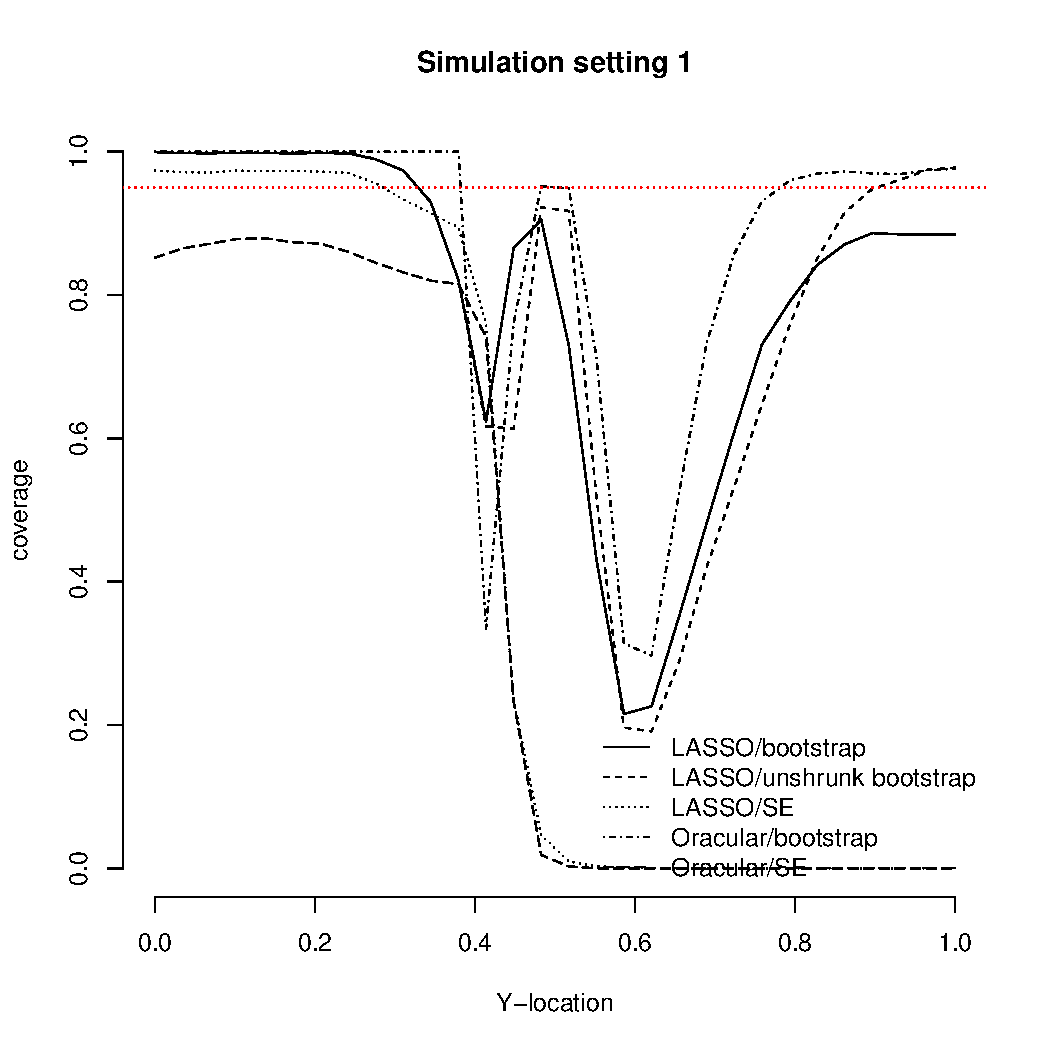
\includegraphics[width=\textwidth]{../../figures/simulation/28-1-profile-coverage.pdf}
			%\caption{A gull}
			\label{fig:gull}
		\end{subfigure}%
        ~ %add desired spacing between images, e. g. ~, \quad, \qquad etc.
          %(or a blank line to force the subfigure onto a new line)
		\begin{subfigure}[b]{0.3\textwidth}
			\centering
			\includegraphics[width=\textwidth]{../../figures/simulation/28-2-profile-coverage.pdf}
			%\caption{A tiger}
			\label{fig:tiger}
		\end{subfigure}
        ~ %add desired spacing between images, e. g. ~, \quad, \qquad etc.
          %(or a blank line to force the subfigure onto a new line)
		\begin{subfigure}[b]{0.3\textwidth}
			\centering
			\includegraphics[width=\textwidth]{../../figures/simulation/28-3-profile-coverage.pdf}
			%\caption{A mouse}
			\label{fig:mouse}
		\end{subfigure}
		%\caption{Pictures of animals}\label{fig:animals}
	\end{figure}
	
	
	\begin{figure}
		\centering
		\begin{subfigure}[b]{0.3\textwidth}
			\centering
			\includegraphics[width=\textwidth]{../../figures/simulation/28-4-profile-coverage.pdf}
			%\caption{A gull}
			\label{fig:gull}
		\end{subfigure}%
        ~ %add desired spacing between images, e. g. ~, \quad, \qquad etc.
          %(or a blank line to force the subfigure onto a new line)
		\begin{subfigure}[b]{0.3\textwidth}
			\centering
			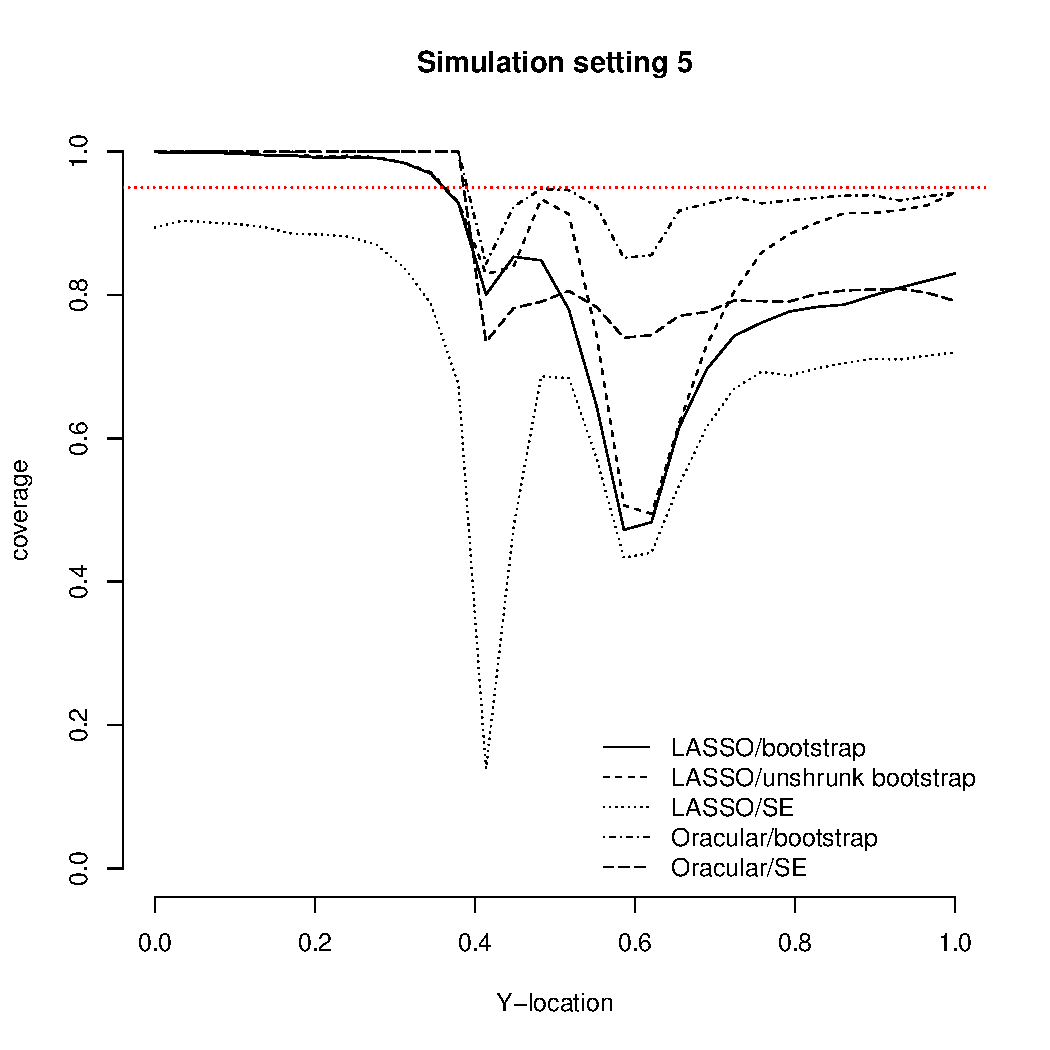
\includegraphics[width=\textwidth]{../../figures/simulation/28-5-profile-coverage.pdf}
			%\caption{A tiger}
			\label{fig:tiger}
		\end{subfigure}
        ~ %add desired spacing between images, e. g. ~, \quad, \qquad etc.
          %(or a blank line to force the subfigure onto a new line)
		\begin{subfigure}[b]{0.3\textwidth}
			\centering
			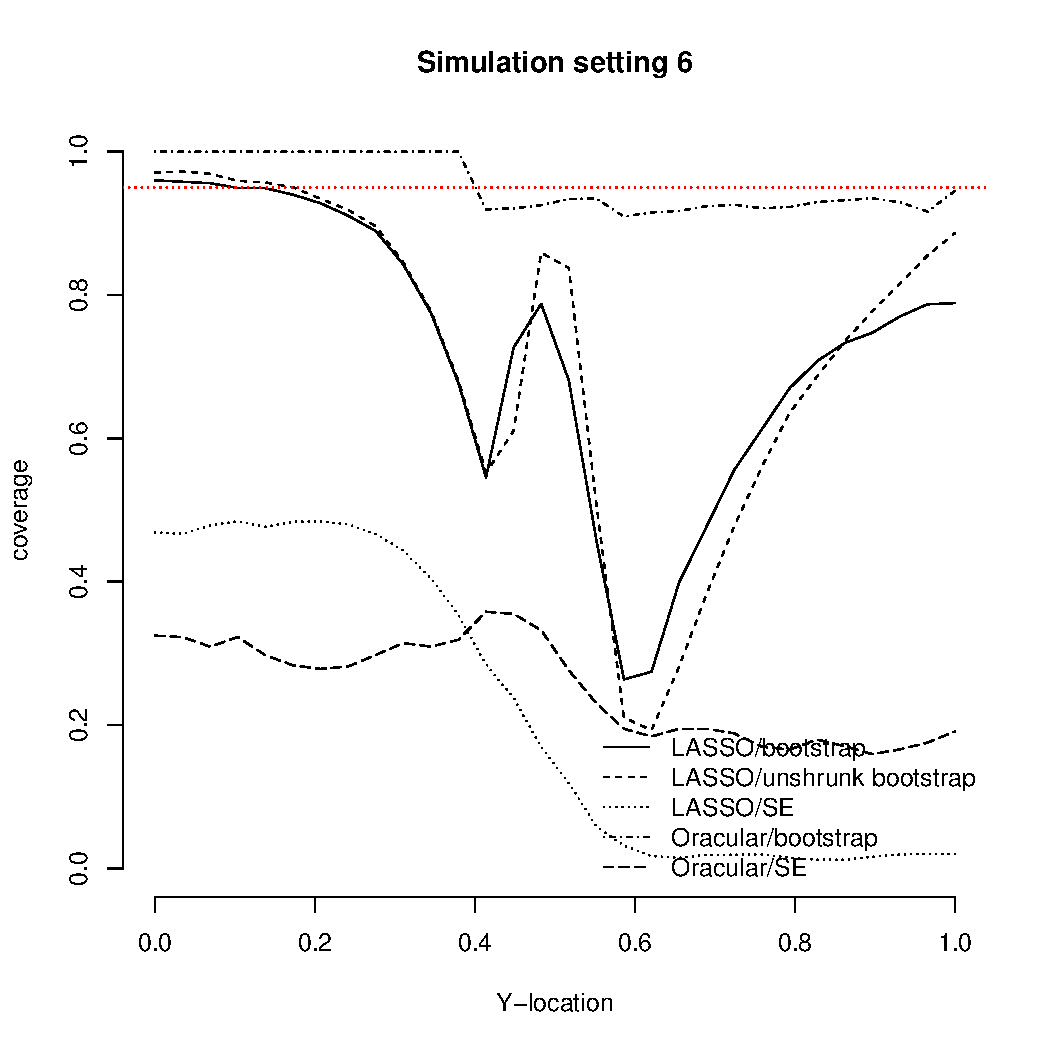
\includegraphics[width=\textwidth]{../../figures/simulation/28-6-profile-coverage.pdf}
			%\caption{A mouse}
			\label{fig:mouse}
		\end{subfigure}
		%\caption{Pictures of animals}\label{fig:animals}
	\end{figure}
	
	
	\begin{figure}
		\centering
		\begin{subfigure}[b]{0.3\textwidth}
			\centering
			\includegraphics[width=\textwidth]{../../figures/simulation/28-7-profile-coverage.pdf}
			%\caption{A gull}
			\label{fig:gull}
		\end{subfigure}%
        ~ %add desired spacing between images, e. g. ~, \quad, \qquad etc.
          %(or a blank line to force the subfigure onto a new line)
		\begin{subfigure}[b]{0.3\textwidth}
			\centering
			\includegraphics[width=\textwidth]{../../figures/simulation/28-8-profile-coverage.pdf}
			\caption{A tiger}
			\label{fig:tiger}
		\end{subfigure}
        ~ %add desired spacing between images, e. g. ~, \quad, \qquad etc.
          %(or a blank line to force the subfigure onto a new line)
		\begin{subfigure}[b]{0.3\textwidth}
			\centering
			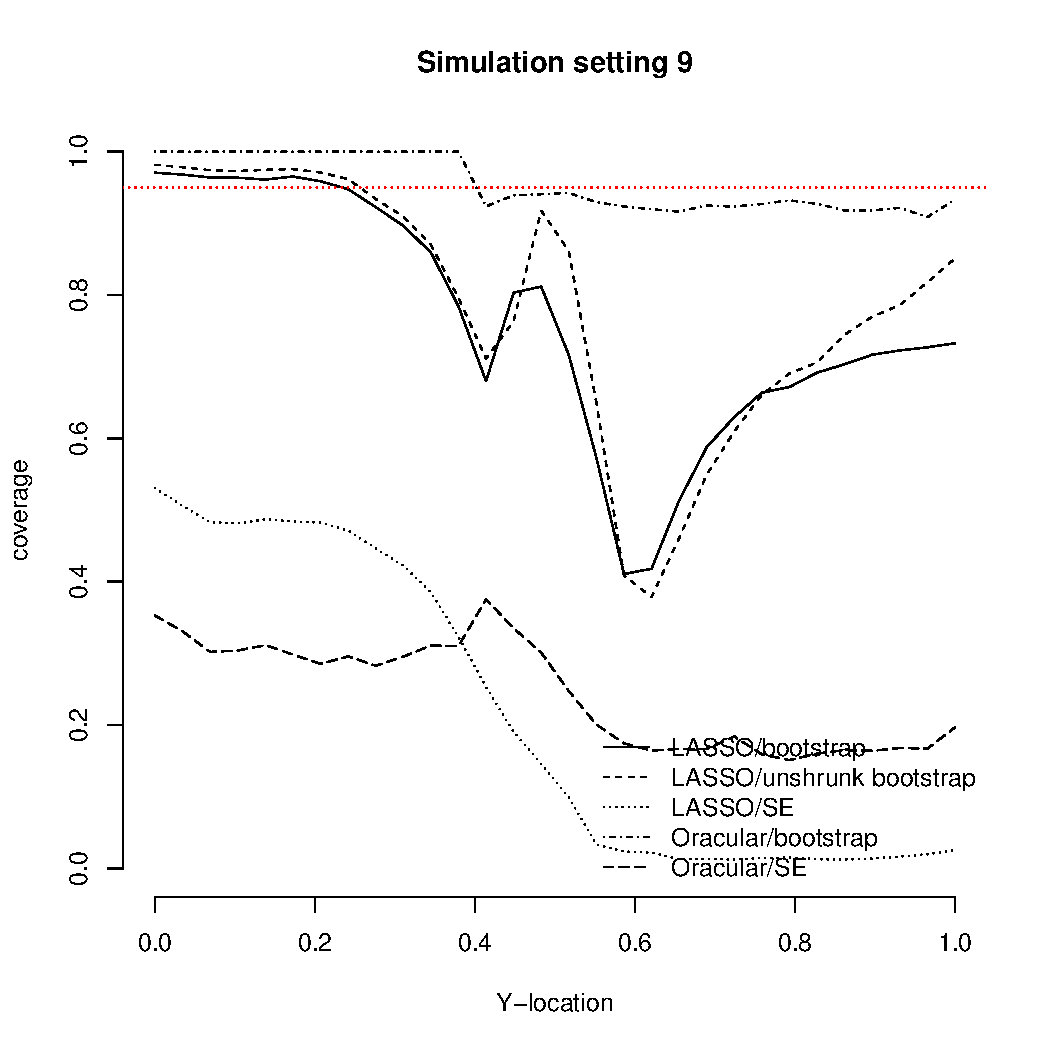
\includegraphics[width=\textwidth]{../../figures/simulation/28-9-profile-coverage.pdf}
			%\caption{A mouse}
			\label{fig:mouse}
		\end{subfigure}
		%\caption{Pictures of animals}\label{fig:animals}
	\end{figure}
	\begin{figure}
		\centering
		\begin{subfigure}[b]{0.3\textwidth}
			\centering
			\includegraphics[width=\textwidth]{../../figures/simulation/28-10-profile-coverage.pdf}
			%\caption{A gull}
			\label{fig:gull}
		\end{subfigure}%
        ~ %add desired spacing between images, e. g. ~, \quad, \qquad etc.
          %(or a blank line to force the subfigure onto a new line)
		\begin{subfigure}[b]{0.3\textwidth}
			\centering
			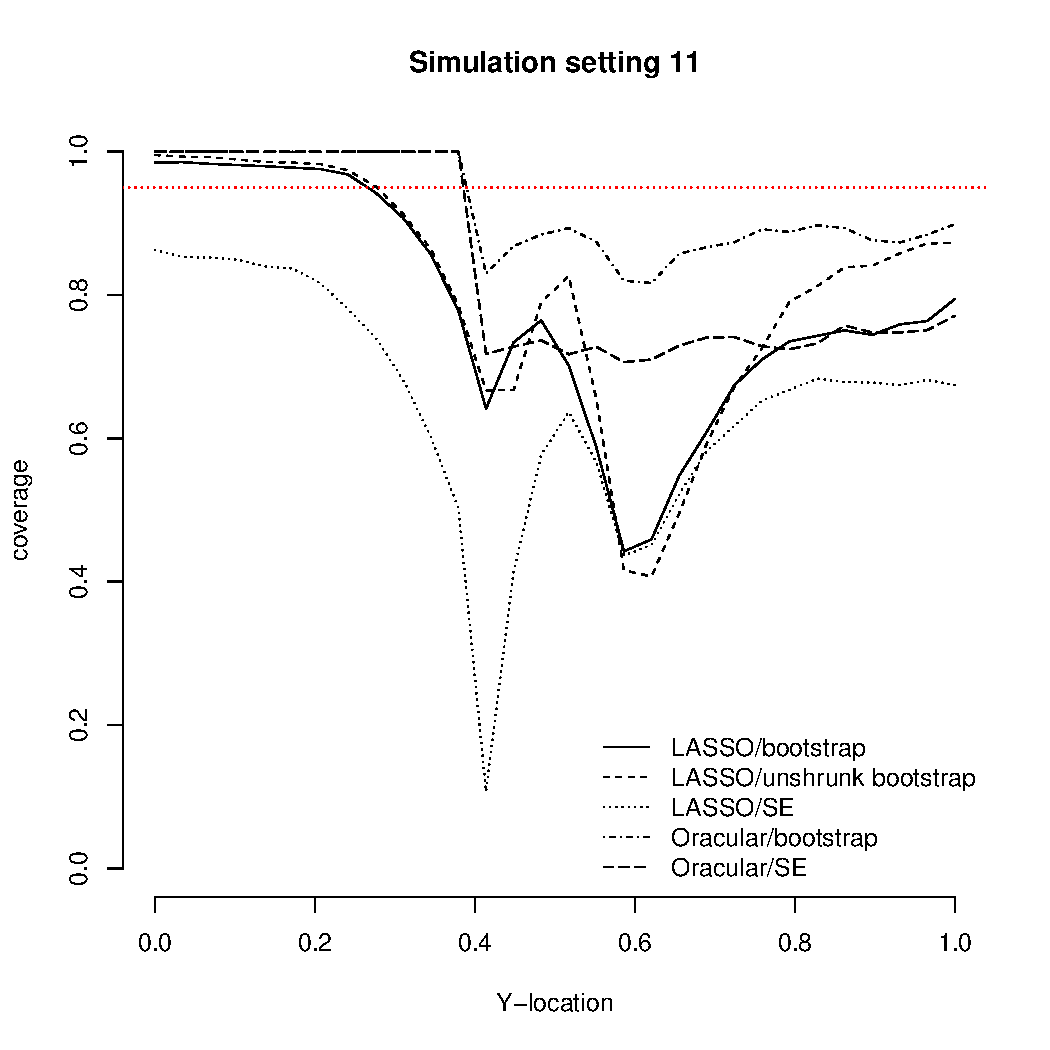
\includegraphics[width=\textwidth]{../../figures/simulation/28-11-profile-coverage.pdf}
			%\caption{A tiger}
			\label{fig:tiger}
		\end{subfigure}
        ~ %add desired spacing between images, e. g. ~, \quad, \qquad etc.
          %(or a blank line to force the subfigure onto a new line)
		\begin{subfigure}[b]{0.3\textwidth}
			\centering
			\includegraphics[width=\textwidth]{../../figures/simulation/28-12-profile-coverage.pdf}
			%\caption{A mouse}
			\label{fig:mouse}
		\end{subfigure}
		%\caption{Pictures of animals}\label{fig:animals}
	\end{figure}
	
	
	\begin{figure}
		\centering
		\begin{subfigure}[b]{0.3\textwidth}
			\centering
			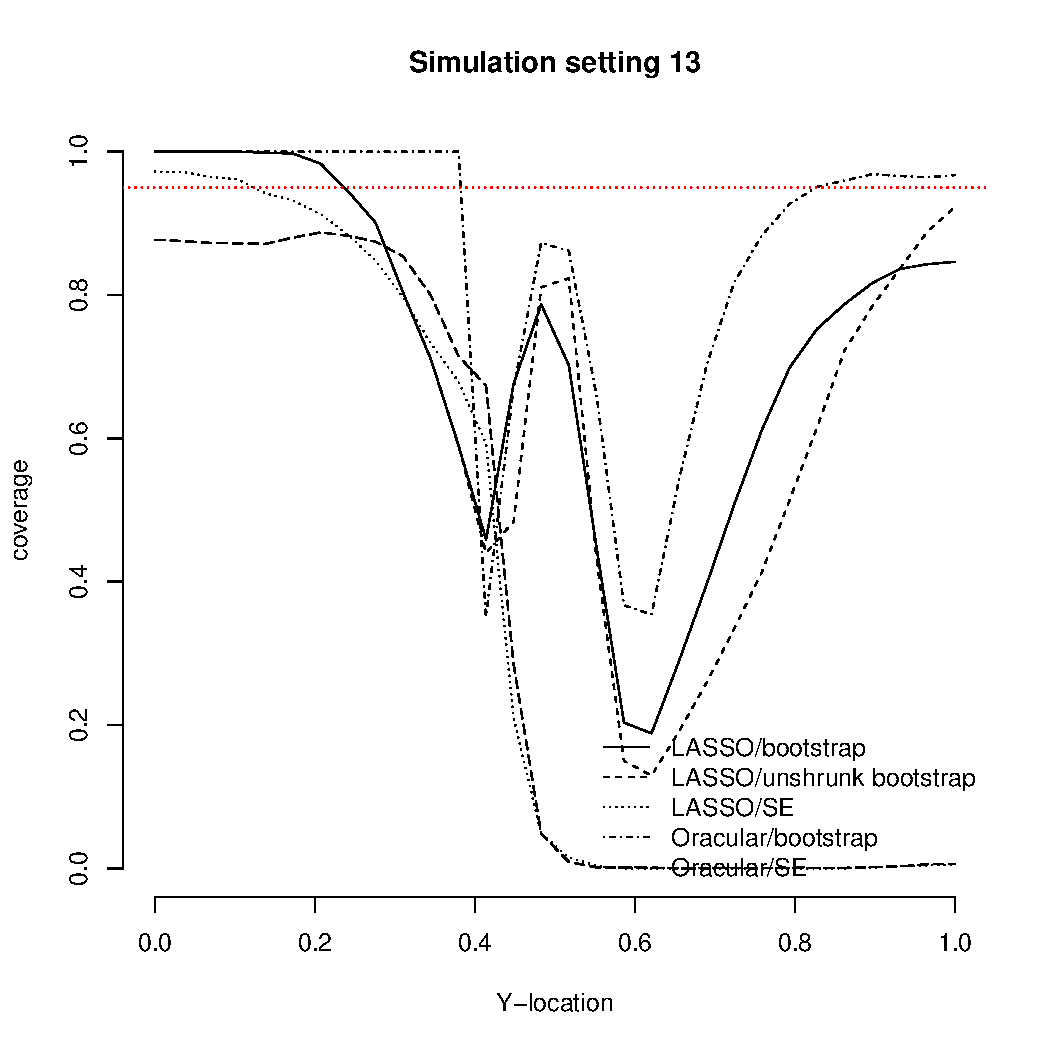
\includegraphics[width=\textwidth]{../../figures/simulation/28-13-profile-coverage.pdf}
			%\caption{A gull}
			\label{fig:gull}
		\end{subfigure}%
        ~ %add desired spacing between images, e. g. ~, \quad, \qquad etc.
          %(or a blank line to force the subfigure onto a new line)
		\begin{subfigure}[b]{0.3\textwidth}
			\centering
			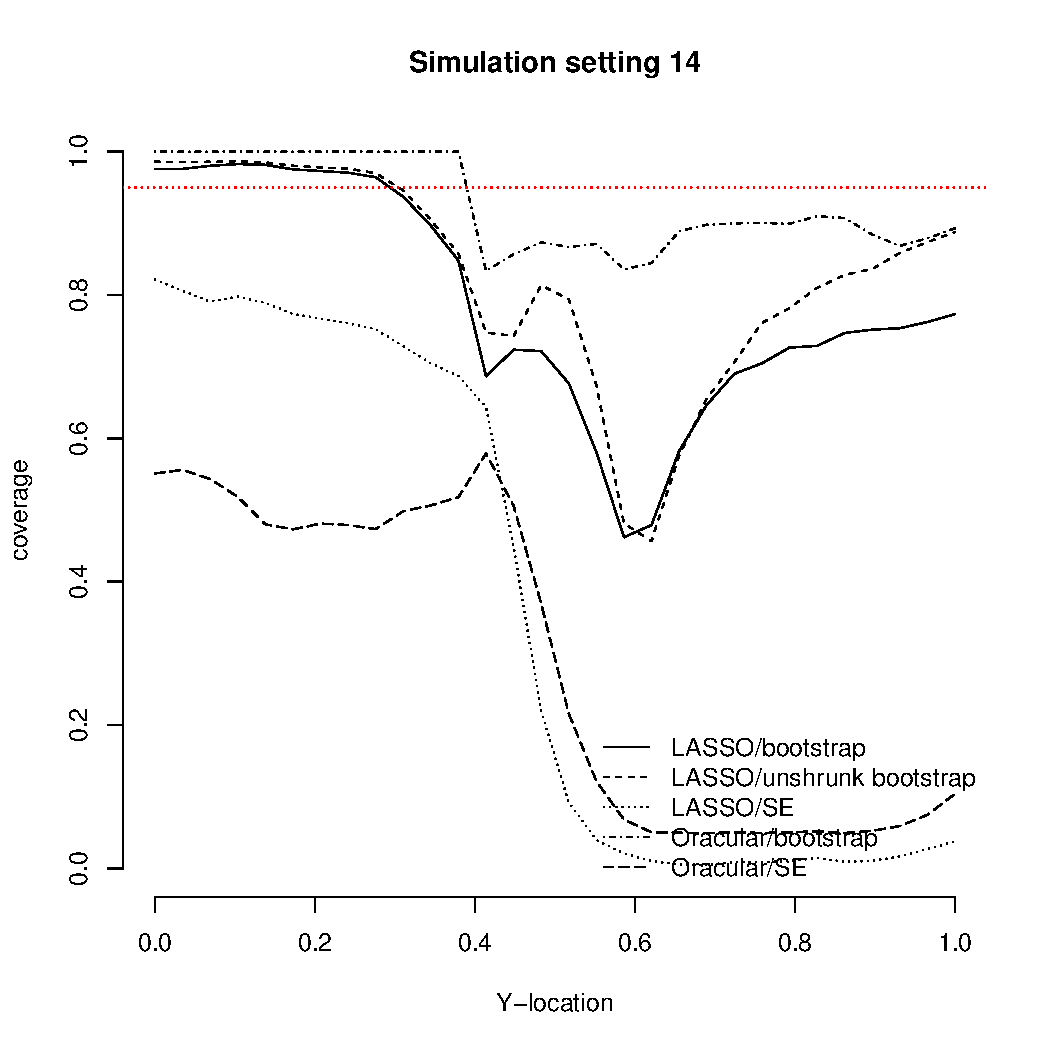
\includegraphics[width=\textwidth]{../../figures/simulation/28-14-profile-coverage.pdf}
			%\caption{A tiger}
			\label{fig:tiger}
		\end{subfigure}
        ~ %add desired spacing between images, e. g. ~, \quad, \qquad etc.
          %(or a blank line to force the subfigure onto a new line)
		\begin{subfigure}[b]{0.3\textwidth}
			\centering
			\includegraphics[width=\textwidth]{../../figures/simulation/28-15-profile-coverage.pdf}
			%\caption{A mouse}
			\label{fig:mouse}
		\end{subfigure}
		%\caption{Pictures of animals}\label{fig:animals}
	\end{figure}
	
	
	\begin{figure}
		\centering
		\begin{subfigure}[b]{0.3\textwidth}
			\centering
			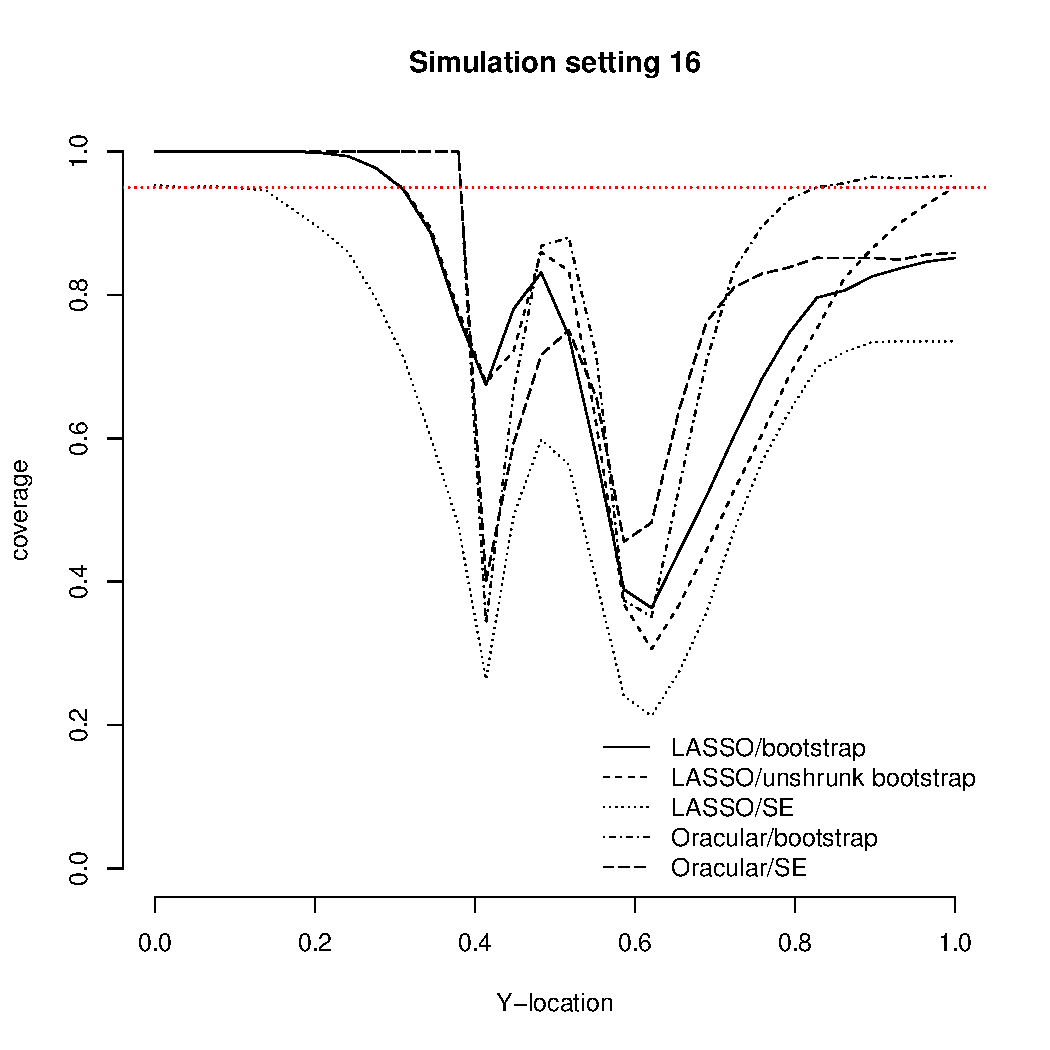
\includegraphics[width=\textwidth]{../../figures/simulation/28-16-profile-coverage.pdf}
			%\caption{A gull}
			\label{fig:gull}
		\end{subfigure}%
        ~ %add desired spacing between images, e. g. ~, \quad, \qquad etc.
          %(or a blank line to force the subfigure onto a new line)
		\begin{subfigure}[b]{0.3\textwidth}
			\centering
			\includegraphics[width=\textwidth]{../../figures/simulation/28-17-profile-coverage.pdf}
			%\caption{A tiger}
			\label{fig:tiger}
		\end{subfigure}
        ~ %add desired spacing between images, e. g. ~, \quad, \qquad etc.
          %(or a blank line to force the subfigure onto a new line)
		\begin{subfigure}[b]{0.3\textwidth}
			\centering
			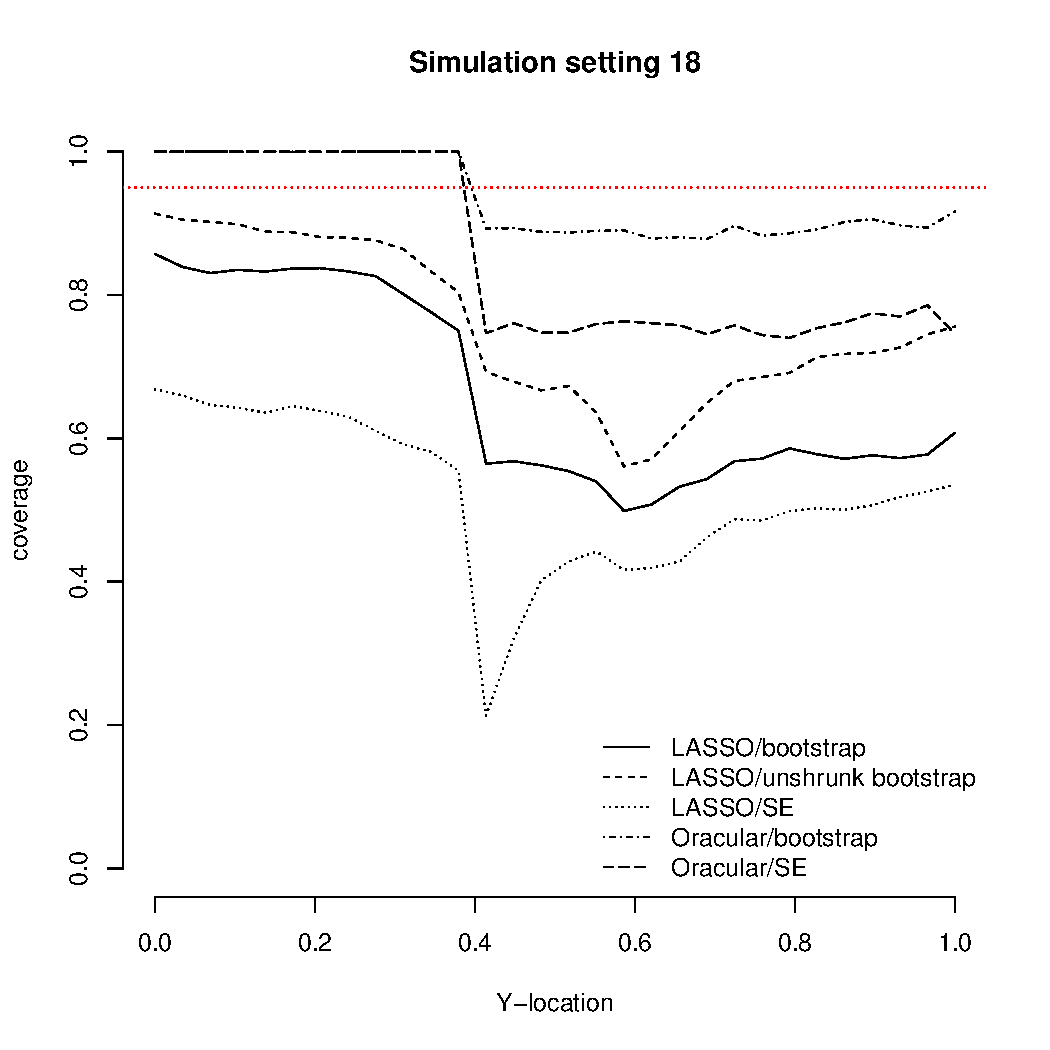
\includegraphics[width=\textwidth]{../../figures/simulation/28-18-profile-coverage.pdf}
			%\caption{A mouse}
			\label{fig:mouse}
		\end{subfigure}
		%\caption{Pictures of animals}\label{fig:animals}
	\end{figure}	
	
	
	
	
	
	\begin{figure}
		\centering
		\begin{subfigure}[b]{0.3\textwidth}
			\centering
			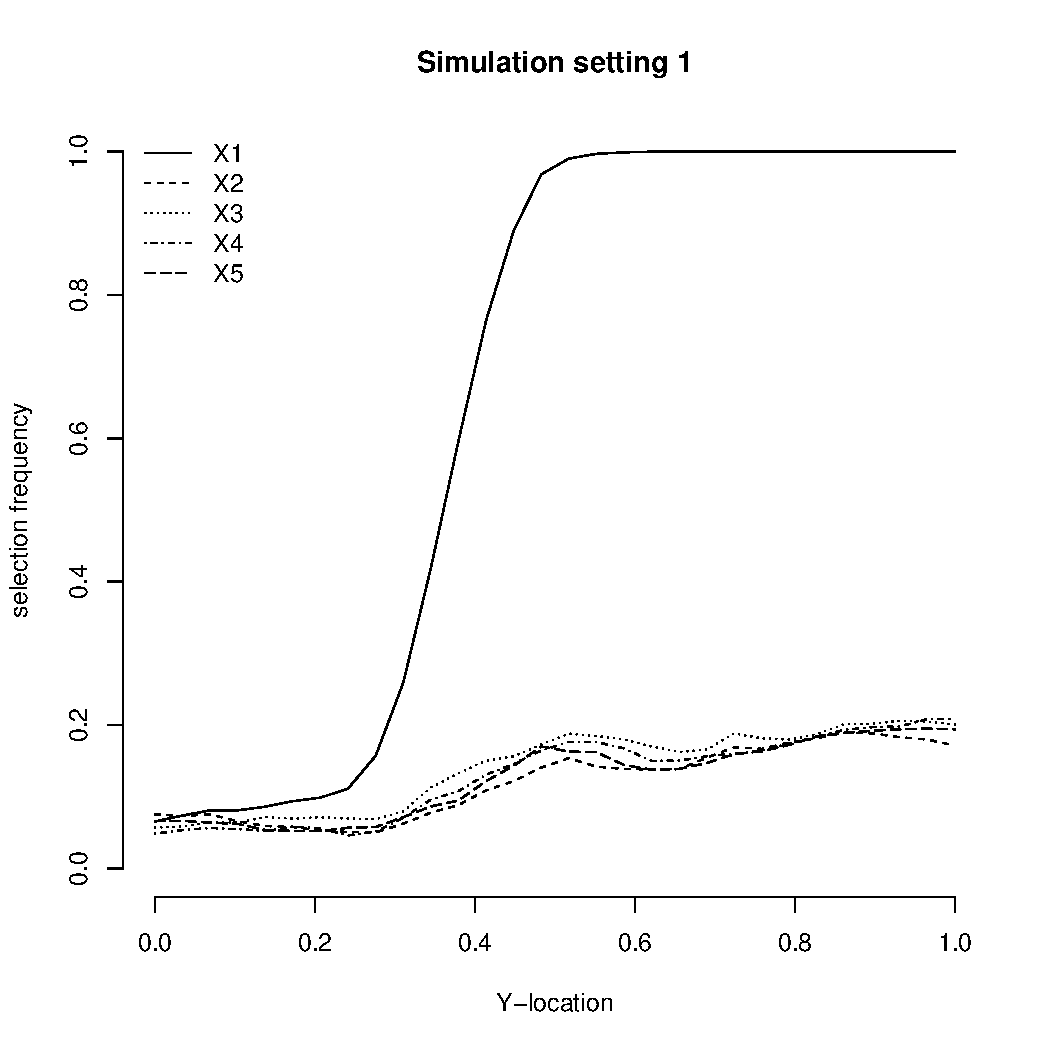
\includegraphics[width=\textwidth]{../../figures/simulation/28-1-profile-selection.pdf}
			%\caption{A gull}
			\label{fig:gull}
		\end{subfigure}%
        ~ %add desired spacing between images, e. g. ~, \quad, \qquad etc.
          %(or a blank line to force the subfigure onto a new line)
		\begin{subfigure}[b]{0.3\textwidth}
			\centering
			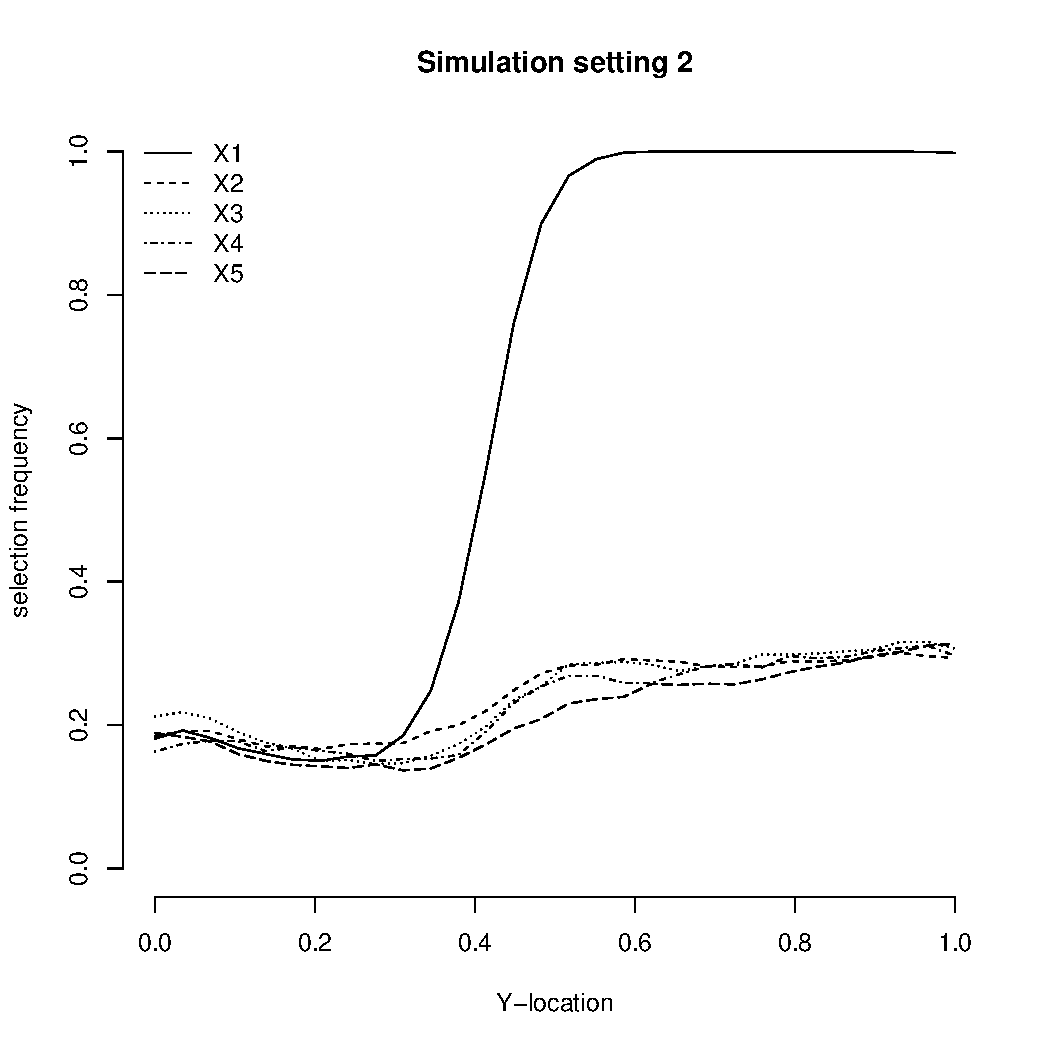
\includegraphics[width=\textwidth]{../../figures/simulation/28-2-profile-selection.pdf}
			%\caption{A tiger}
			\label{fig:tiger}
		\end{subfigure}
        ~ %add desired spacing between images, e. g. ~, \quad, \qquad etc.
          %(or a blank line to force the subfigure onto a new line)
		\begin{subfigure}[b]{0.3\textwidth}
			\centering
			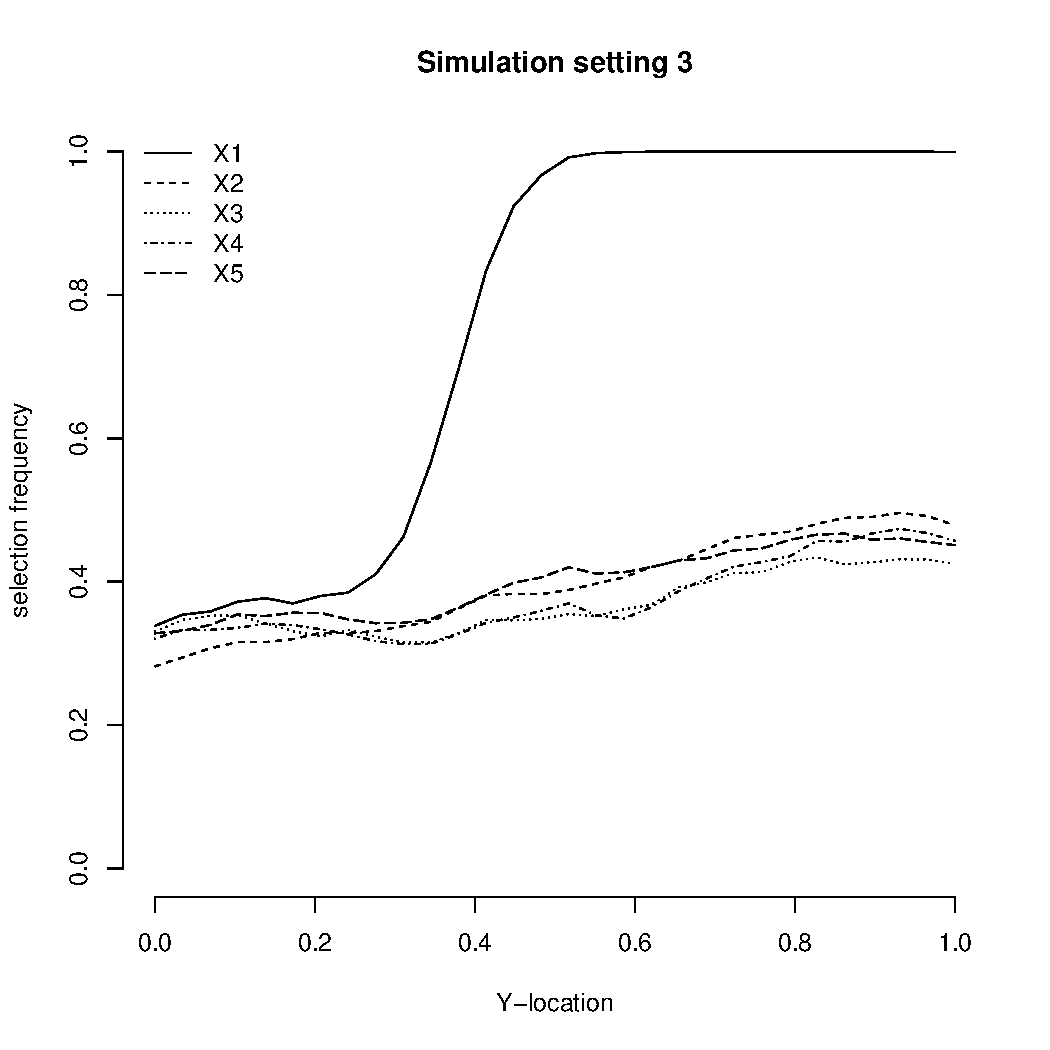
\includegraphics[width=\textwidth]{../../figures/simulation/28-3-profile-selection.pdf}
			%\caption{A mouse}
			\label{fig:mouse}
		\end{subfigure}
		%\caption{Pictures of animals}\label{fig:animals}
	\end{figure}
	
	
	\begin{figure}
		\centering
		\begin{subfigure}[b]{0.3\textwidth}
			\centering
			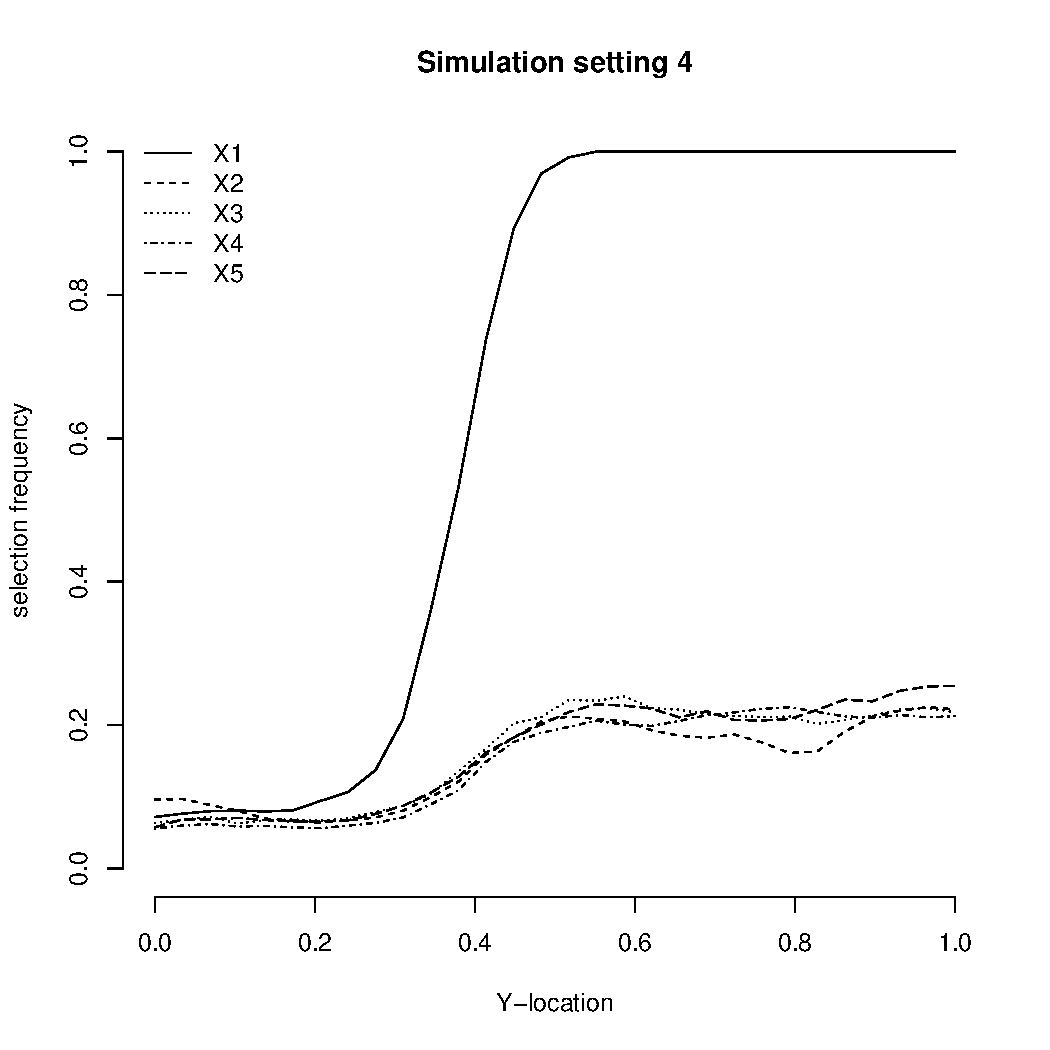
\includegraphics[width=\textwidth]{../../figures/simulation/28-4-profile-selection.pdf}
			%\caption{A gull}
			\label{fig:gull}
		\end{subfigure}%
        ~ %add desired spacing between images, e. g. ~, \quad, \qquad etc.
          %(or a blank line to force the subfigure onto a new line)
		\begin{subfigure}[b]{0.3\textwidth}
			\centering
			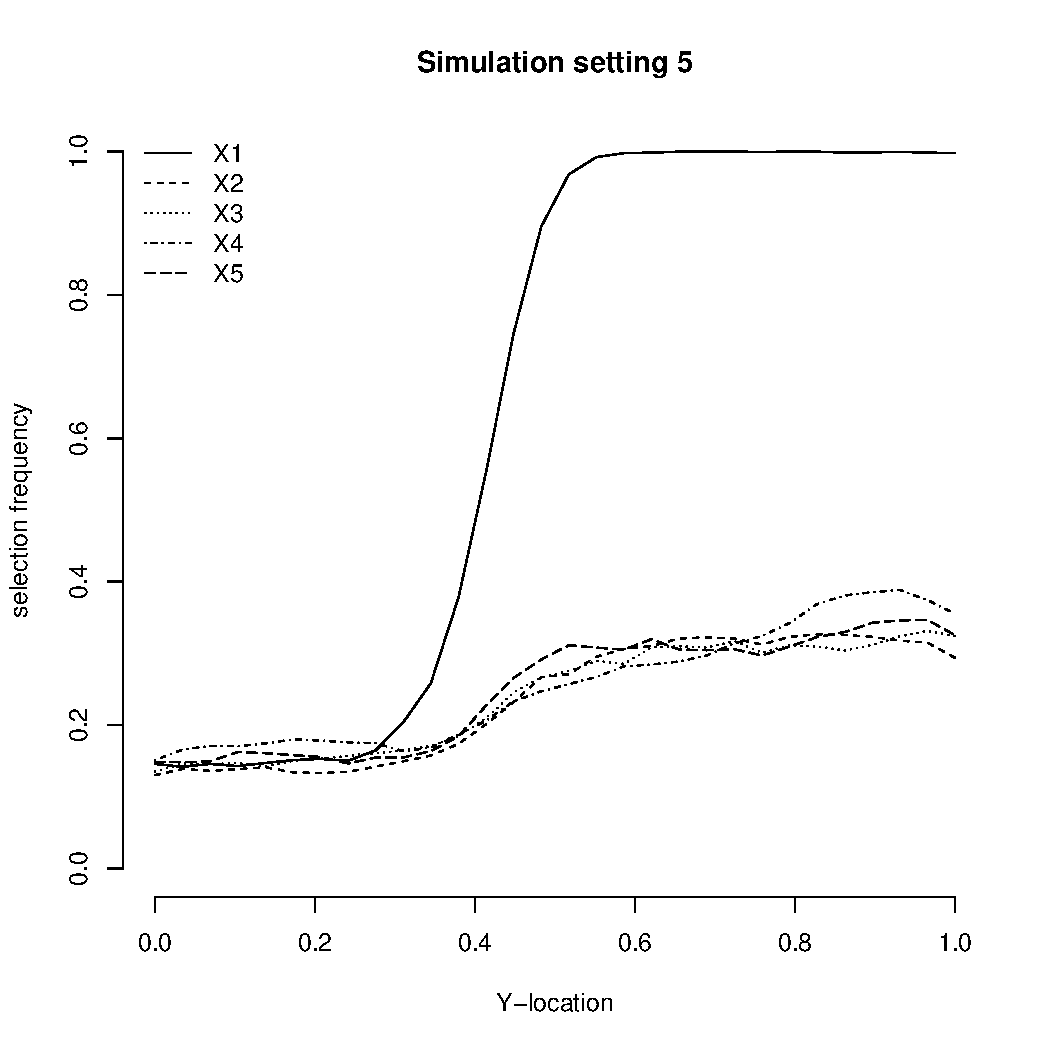
\includegraphics[width=\textwidth]{../../figures/simulation/28-5-profile-selection.pdf}
			%\caption{A tiger}
			\label{fig:tiger}
		\end{subfigure}
        ~ %add desired spacing between images, e. g. ~, \quad, \qquad etc.
          %(or a blank line to force the subfigure onto a new line)
		\begin{subfigure}[b]{0.3\textwidth}
			\centering
			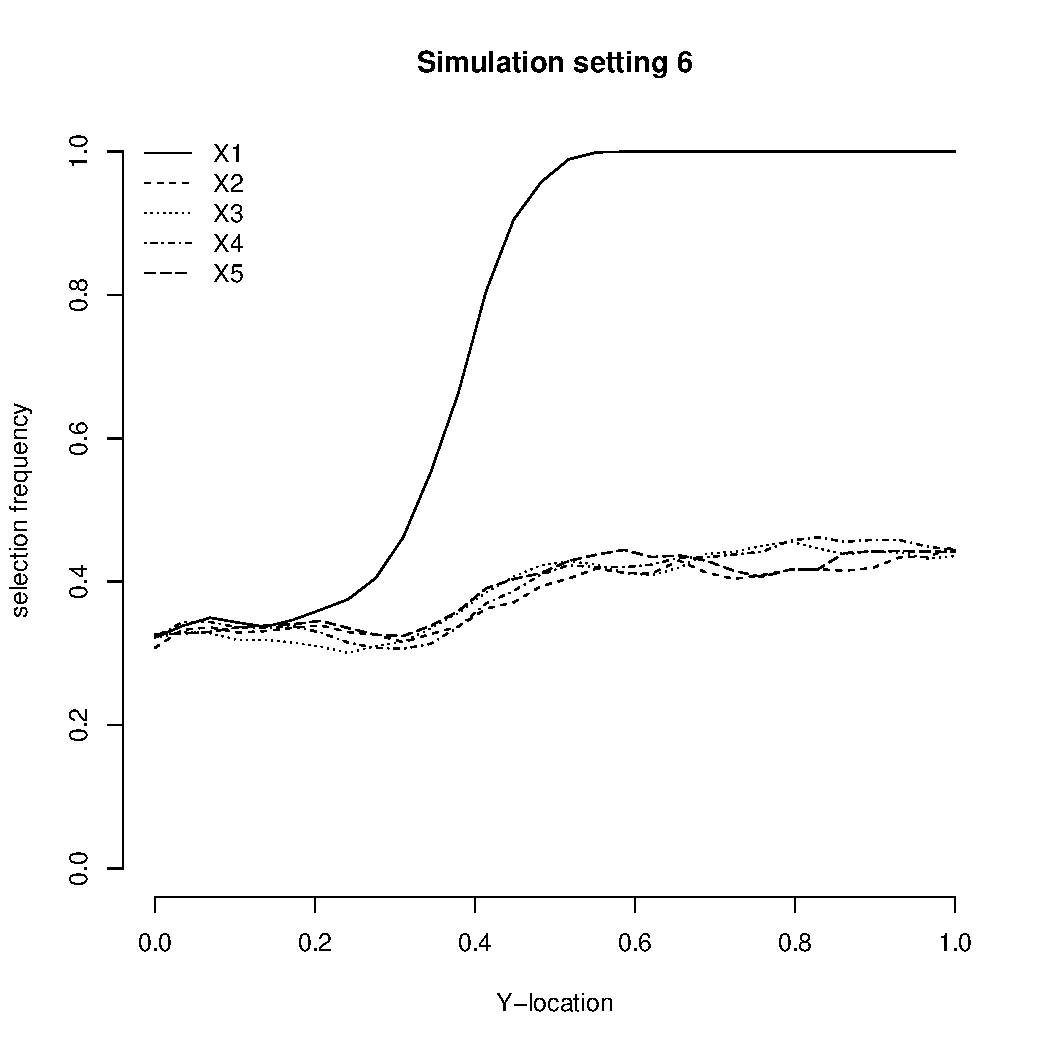
\includegraphics[width=\textwidth]{../../figures/simulation/28-6-profile-selection.pdf}
			%\caption{A mouse}
			\label{fig:mouse}
		\end{subfigure}
		%\caption{Pictures of animals}\label{fig:animals}
	\end{figure}
	
	
	\begin{figure}
		\centering
		\begin{subfigure}[b]{0.3\textwidth}
			\centering
			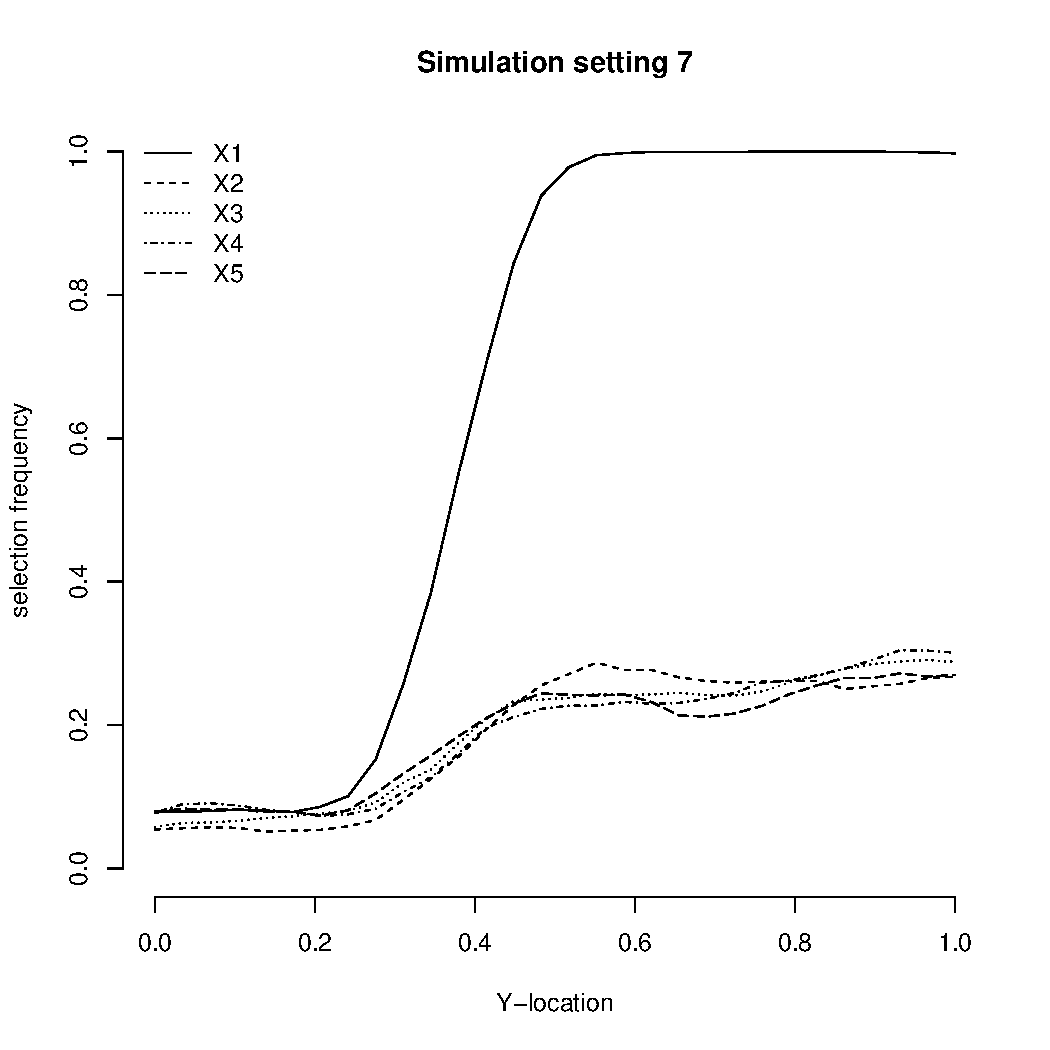
\includegraphics[width=\textwidth]{../../figures/simulation/28-7-profile-selection.pdf}
			%\caption{A gull}
			\label{fig:gull}
		\end{subfigure}%
        ~ %add desired spacing between images, e. g. ~, \quad, \qquad etc.
          %(or a blank line to force the subfigure onto a new line)
		\begin{subfigure}[b]{0.3\textwidth}
			\centering
			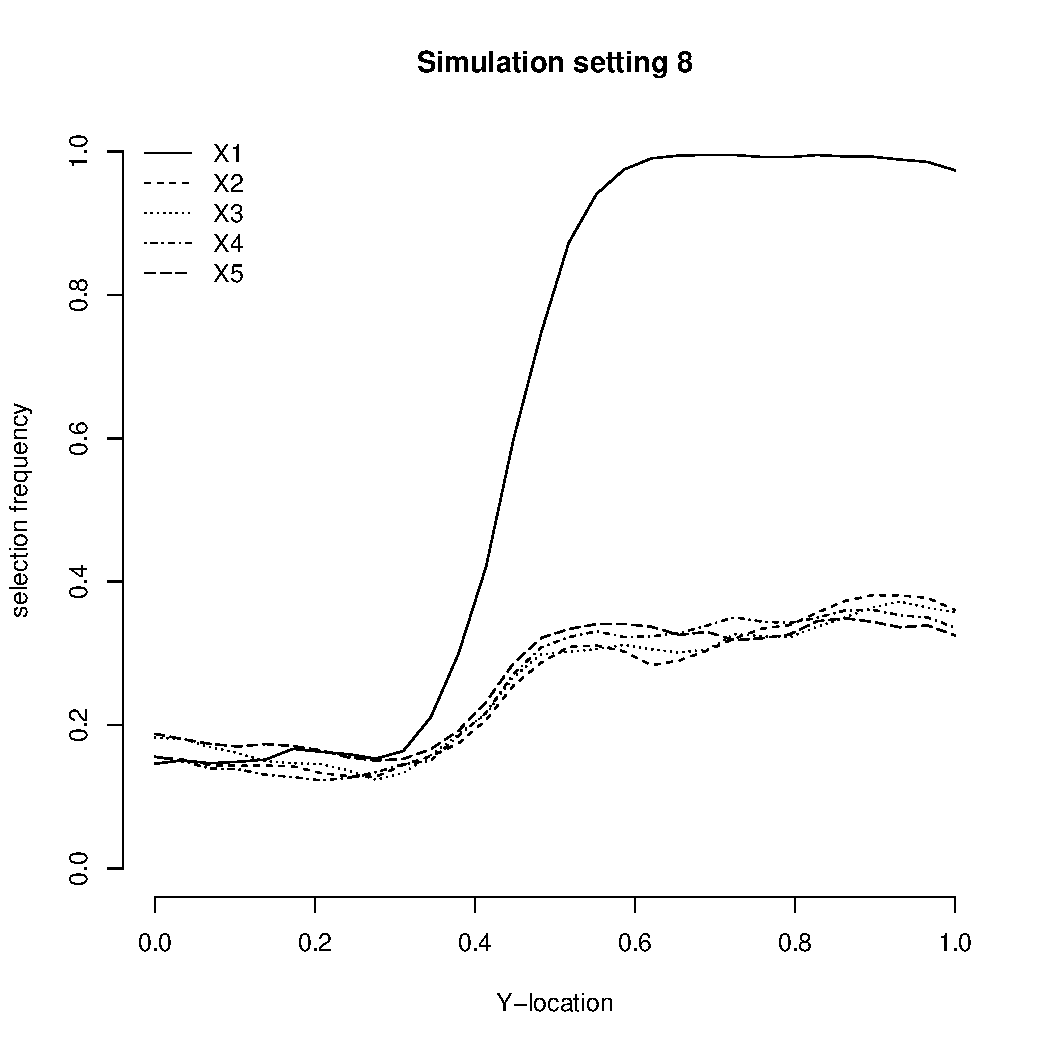
\includegraphics[width=\textwidth]{../../figures/simulation/28-8-profile-selection.pdf}
			\caption{A tiger}
			\label{fig:tiger}
		\end{subfigure}
        ~ %add desired spacing between images, e. g. ~, \quad, \qquad etc.
          %(or a blank line to force the subfigure onto a new line)
		\begin{subfigure}[b]{0.3\textwidth}
			\centering
			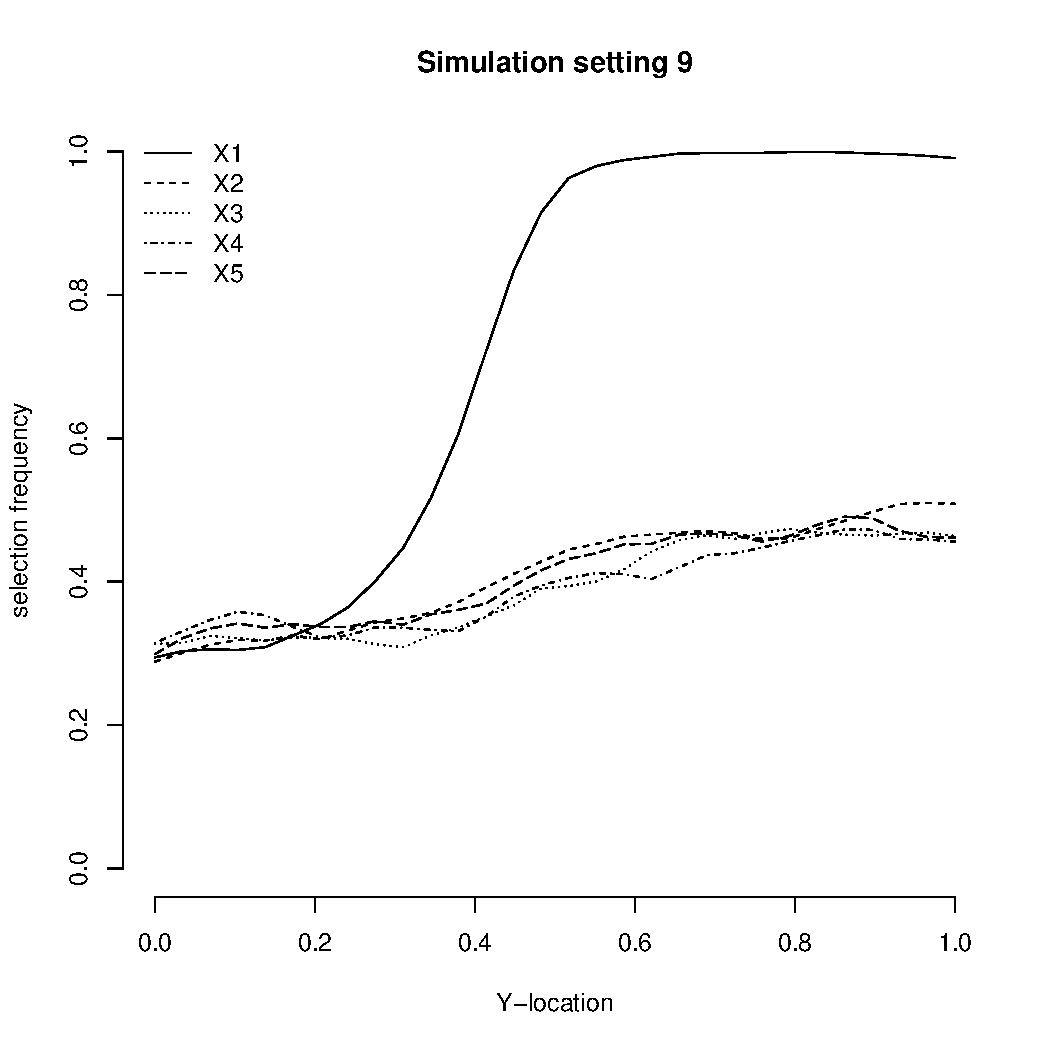
\includegraphics[width=\textwidth]{../../figures/simulation/28-9-profile-selection.pdf}
			%\caption{A mouse}
			\label{fig:mouse}
		\end{subfigure}
		%\caption{Pictures of animals}\label{fig:animals}
	\end{figure}
	\begin{figure}
		\centering
		\begin{subfigure}[b]{0.3\textwidth}
			\centering
			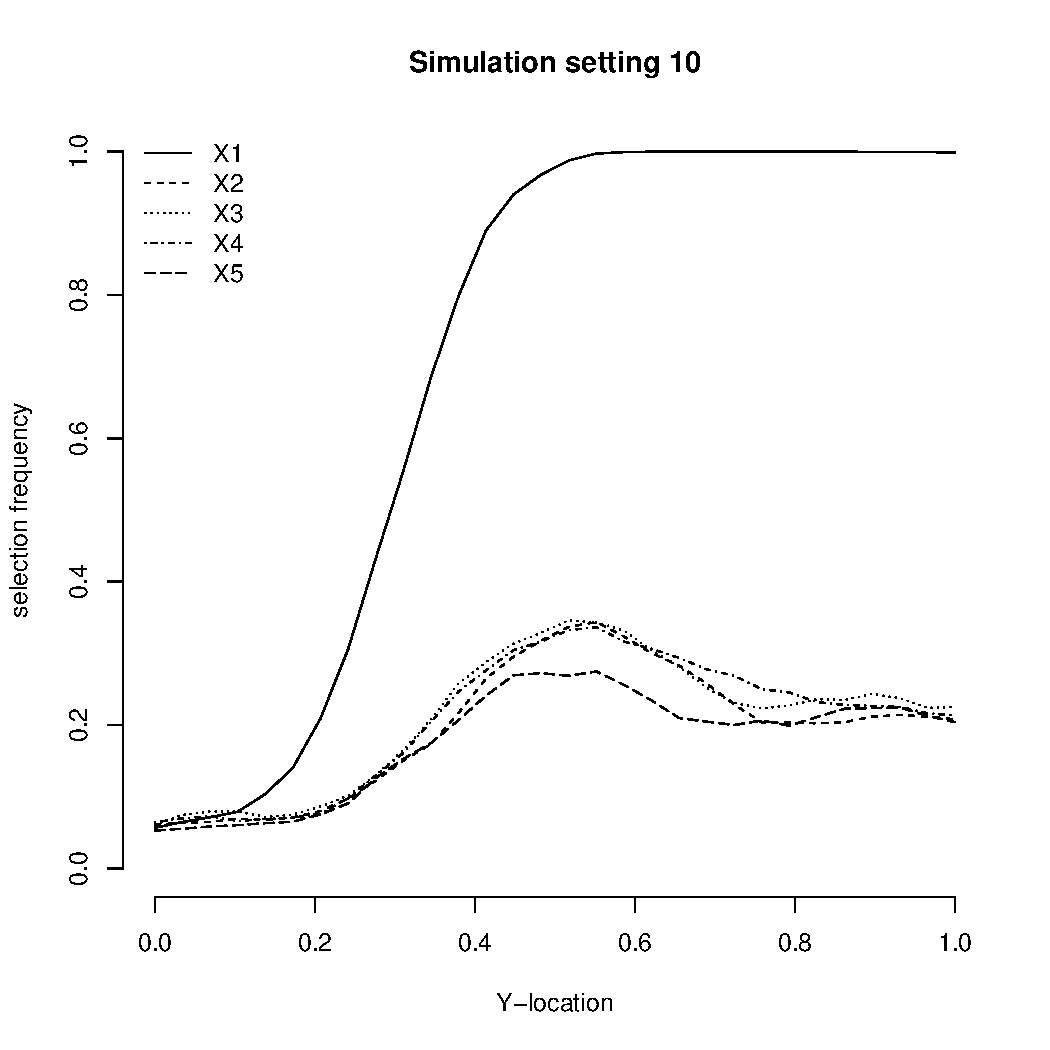
\includegraphics[width=\textwidth]{../../figures/simulation/28-10-profile-selection.pdf}
			%\caption{A gull}
			\label{fig:gull}
		\end{subfigure}%
        ~ %add desired spacing between images, e. g. ~, \quad, \qquad etc.
          %(or a blank line to force the subfigure onto a new line)
		\begin{subfigure}[b]{0.3\textwidth}
			\centering
			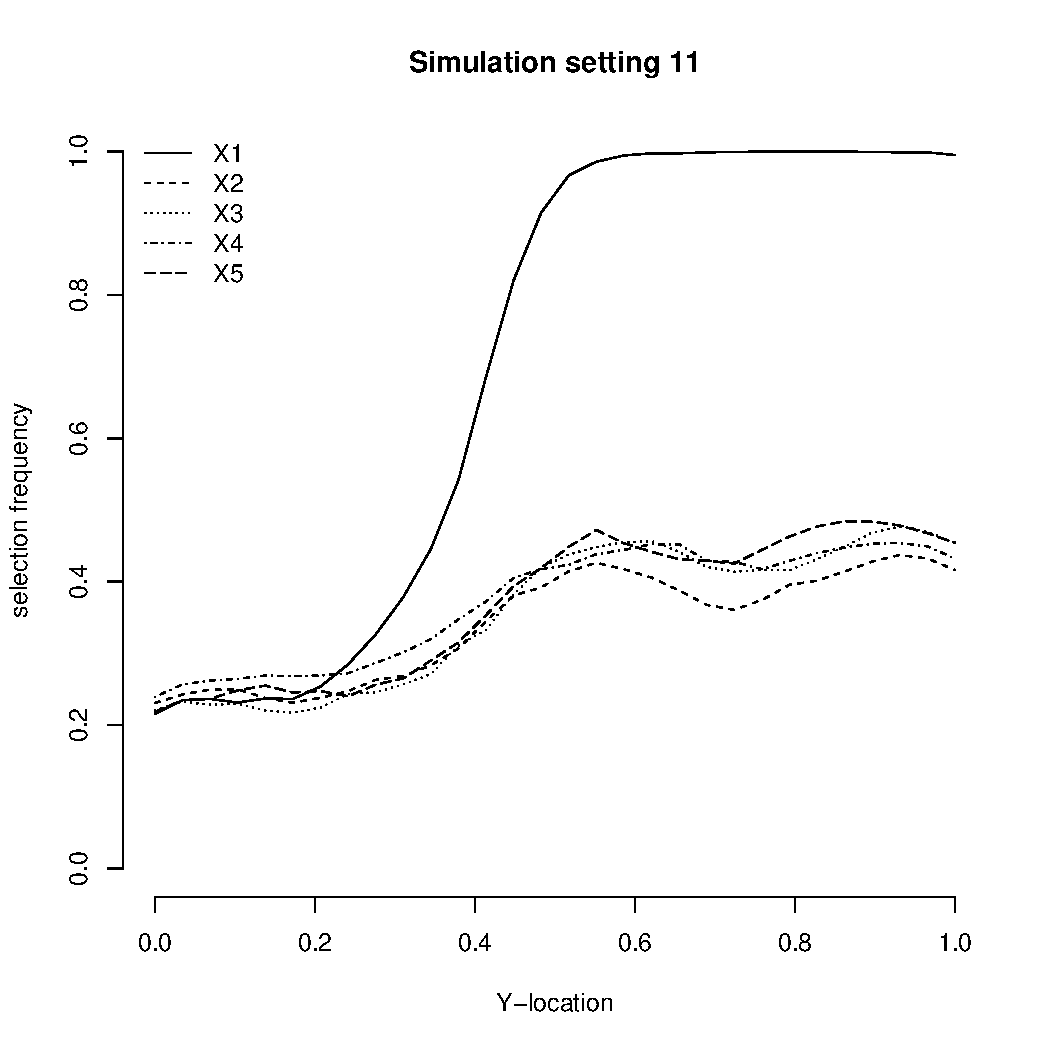
\includegraphics[width=\textwidth]{../../figures/simulation/28-11-profile-selection.pdf}
			%\caption{A tiger}
			\label{fig:tiger}
		\end{subfigure}
        ~ %add desired spacing between images, e. g. ~, \quad, \qquad etc.
          %(or a blank line to force the subfigure onto a new line)
		\begin{subfigure}[b]{0.3\textwidth}
			\centering
			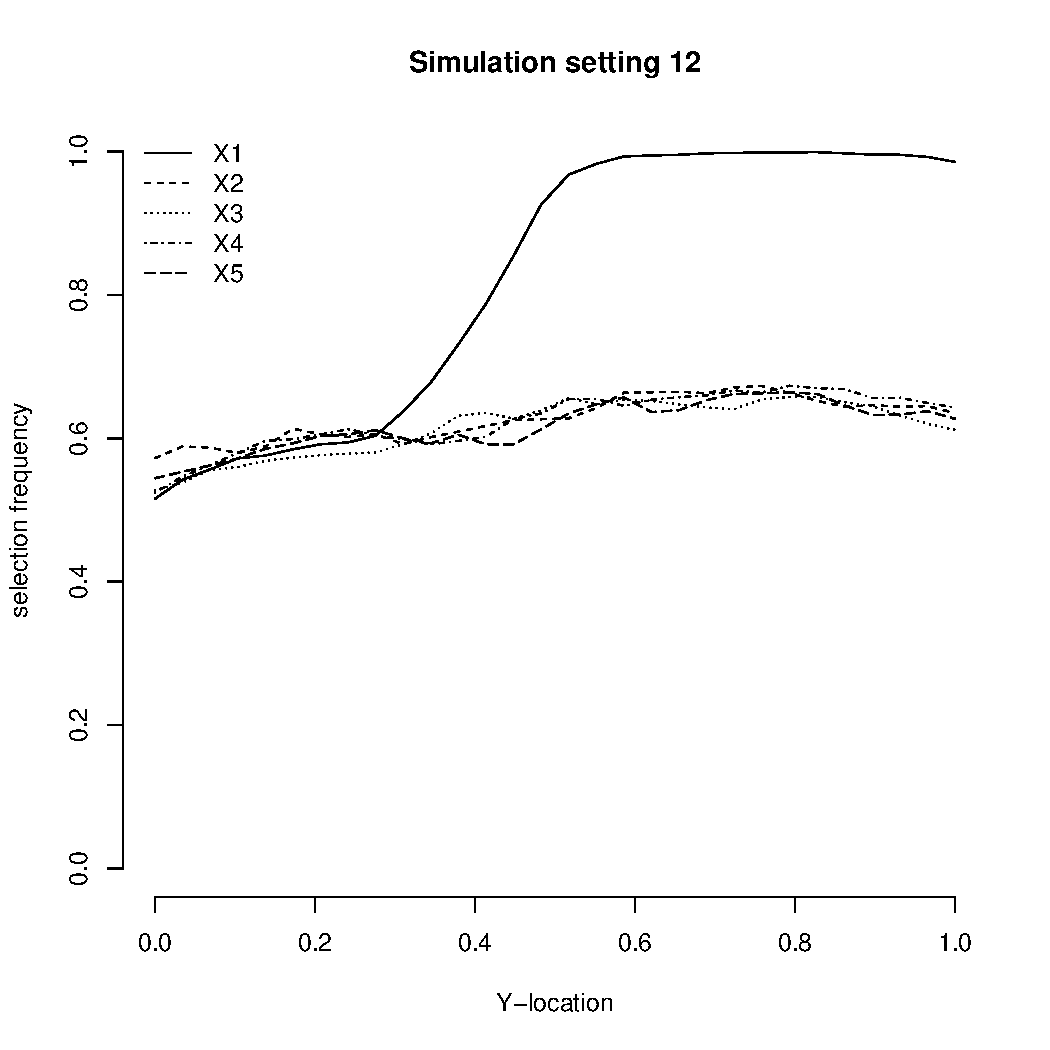
\includegraphics[width=\textwidth]{../../figures/simulation/28-12-profile-selection.pdf}
			%\caption{A mouse}
			\label{fig:mouse}
		\end{subfigure}
		%\caption{Pictures of animals}\label{fig:animals}
	\end{figure}
	
	
	\begin{figure}
		\centering
		\begin{subfigure}[b]{0.3\textwidth}
			\centering
			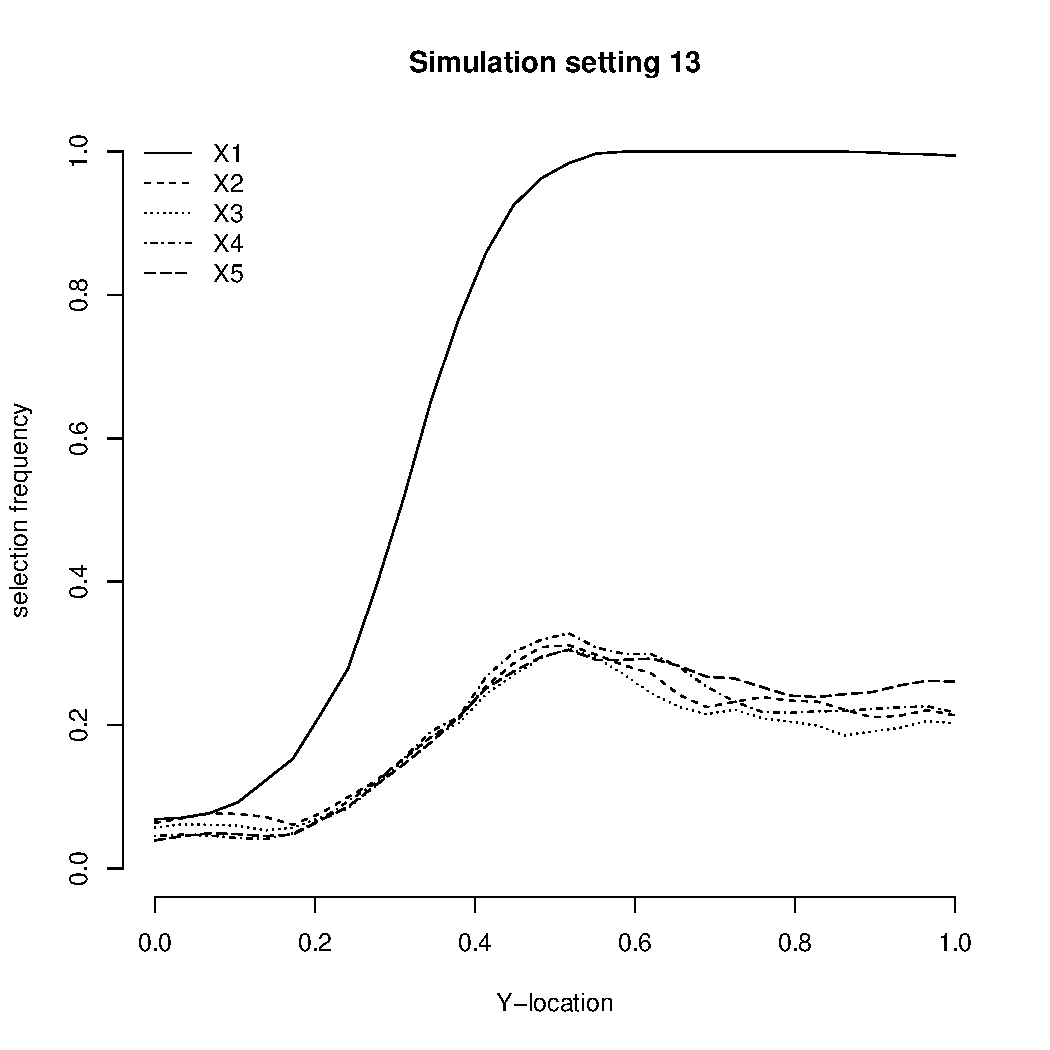
\includegraphics[width=\textwidth]{../../figures/simulation/28-13-profile-selection.pdf}
			%\caption{A gull}
			\label{fig:gull}
		\end{subfigure}%
        ~ %add desired spacing between images, e. g. ~, \quad, \qquad etc.
          %(or a blank line to force the subfigure onto a new line)
		\begin{subfigure}[b]{0.3\textwidth}
			\centering
			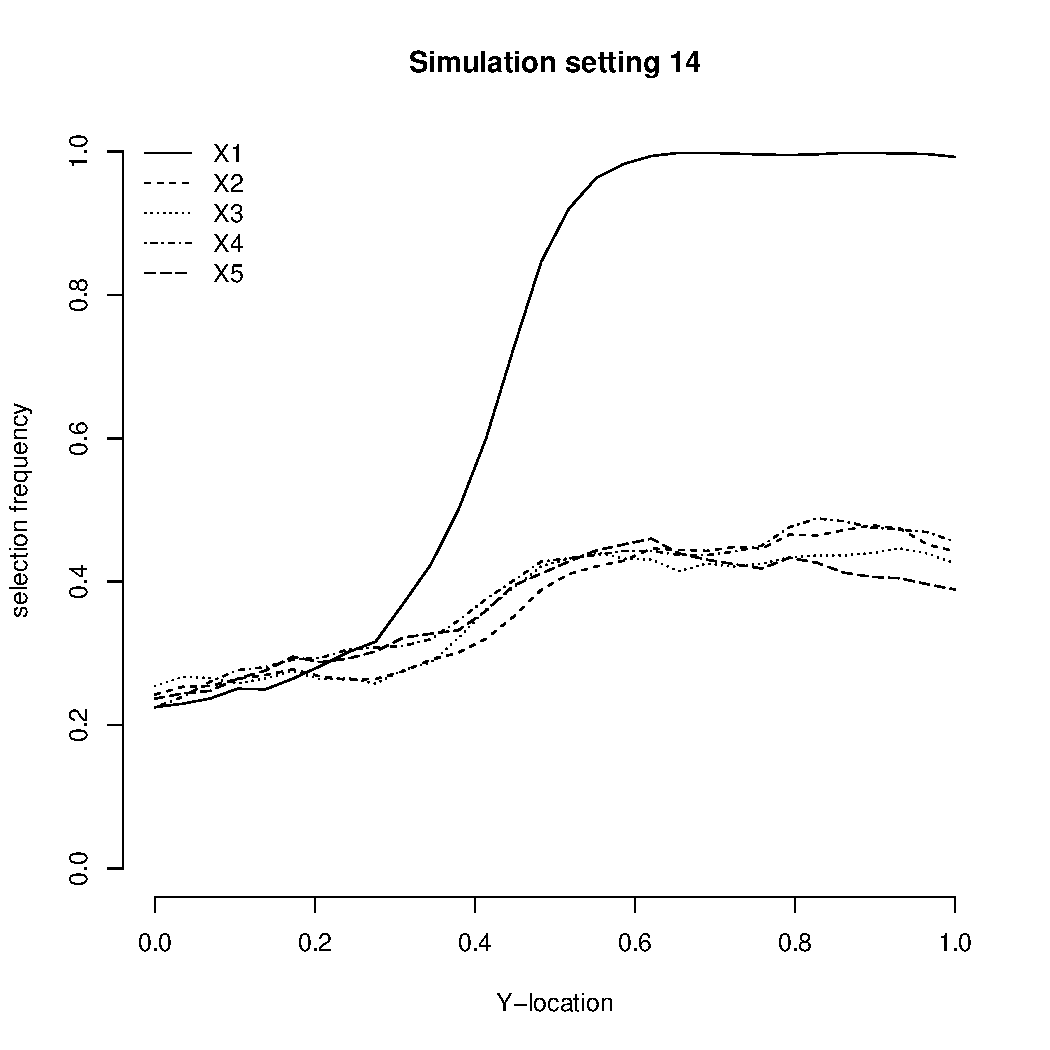
\includegraphics[width=\textwidth]{../../figures/simulation/28-14-profile-selection.pdf}
			%\caption{A tiger}
			\label{fig:tiger}
		\end{subfigure}
        ~ %add desired spacing between images, e. g. ~, \quad, \qquad etc.
          %(or a blank line to force the subfigure onto a new line)
		\begin{subfigure}[b]{0.3\textwidth}
			\centering
			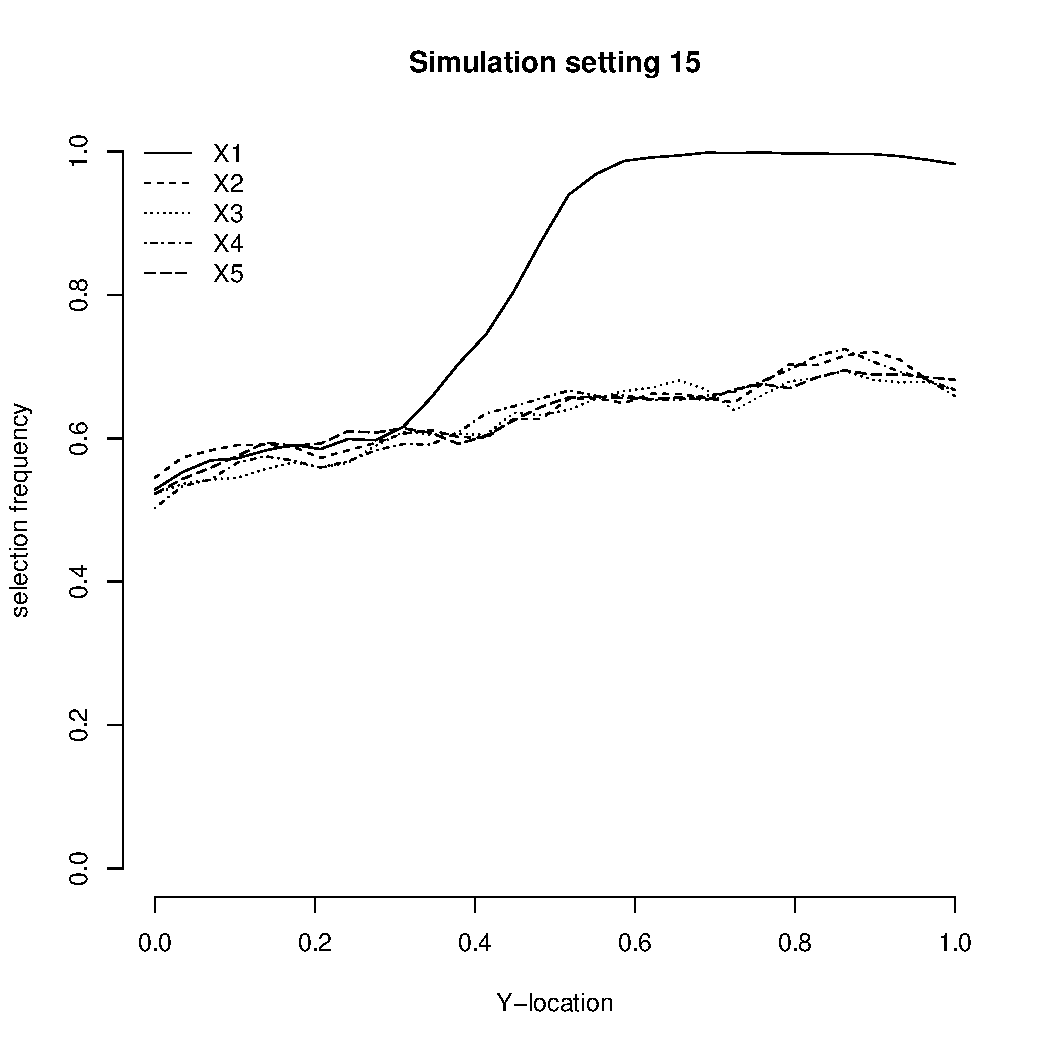
\includegraphics[width=\textwidth]{../../figures/simulation/28-15-profile-selection.pdf}
			%\caption{A mouse}
			\label{fig:mouse}
		\end{subfigure}
		%\caption{Pictures of animals}\label{fig:animals}
	\end{figure}
	
	
	\begin{figure}
		\centering
		\begin{subfigure}[b]{0.3\textwidth}
			\centering
			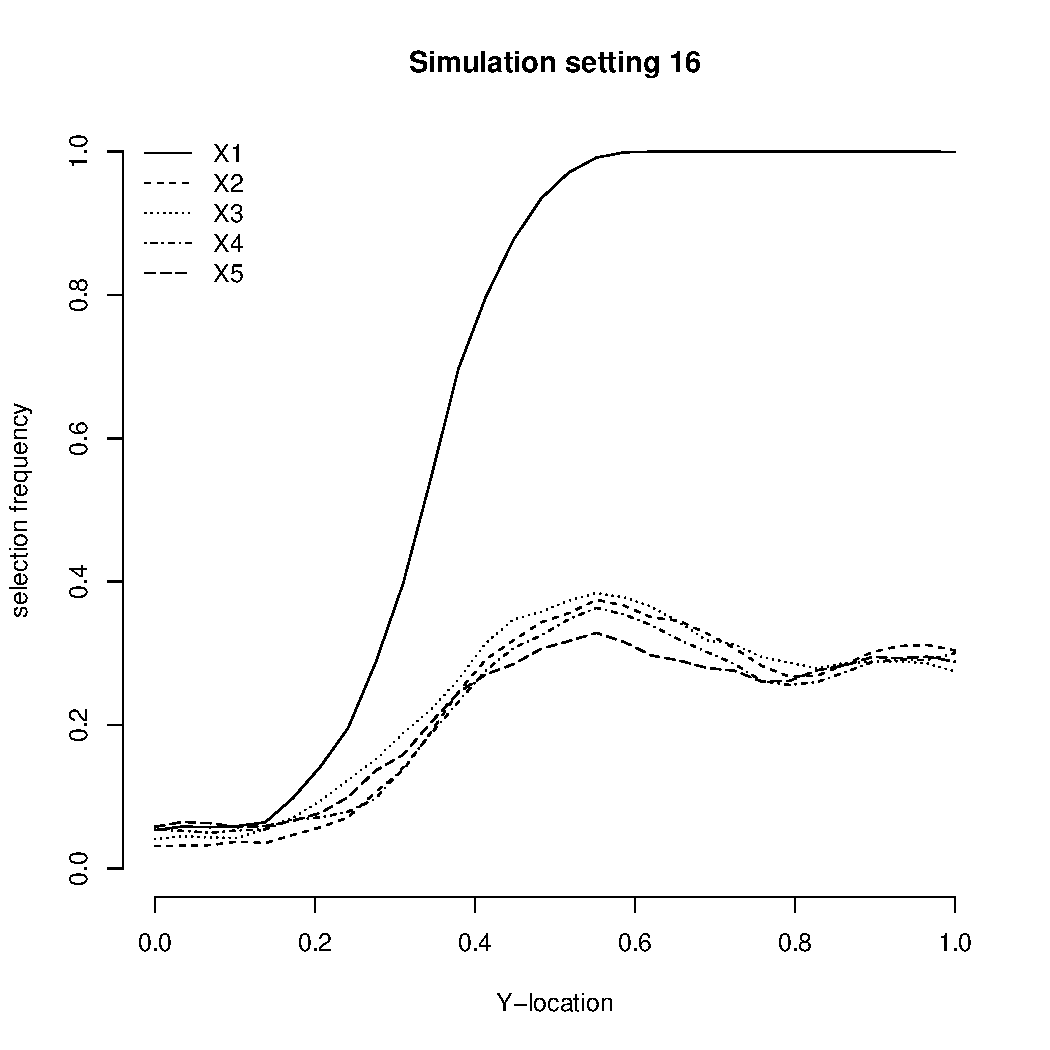
\includegraphics[width=\textwidth]{../../figures/simulation/28-16-profile-selection.pdf}
			%\caption{A gull}
			\label{fig:gull}
		\end{subfigure}%
        ~ %add desired spacing between images, e. g. ~, \quad, \qquad etc.
          %(or a blank line to force the subfigure onto a new line)
		\begin{subfigure}[b]{0.3\textwidth}
			\centering
			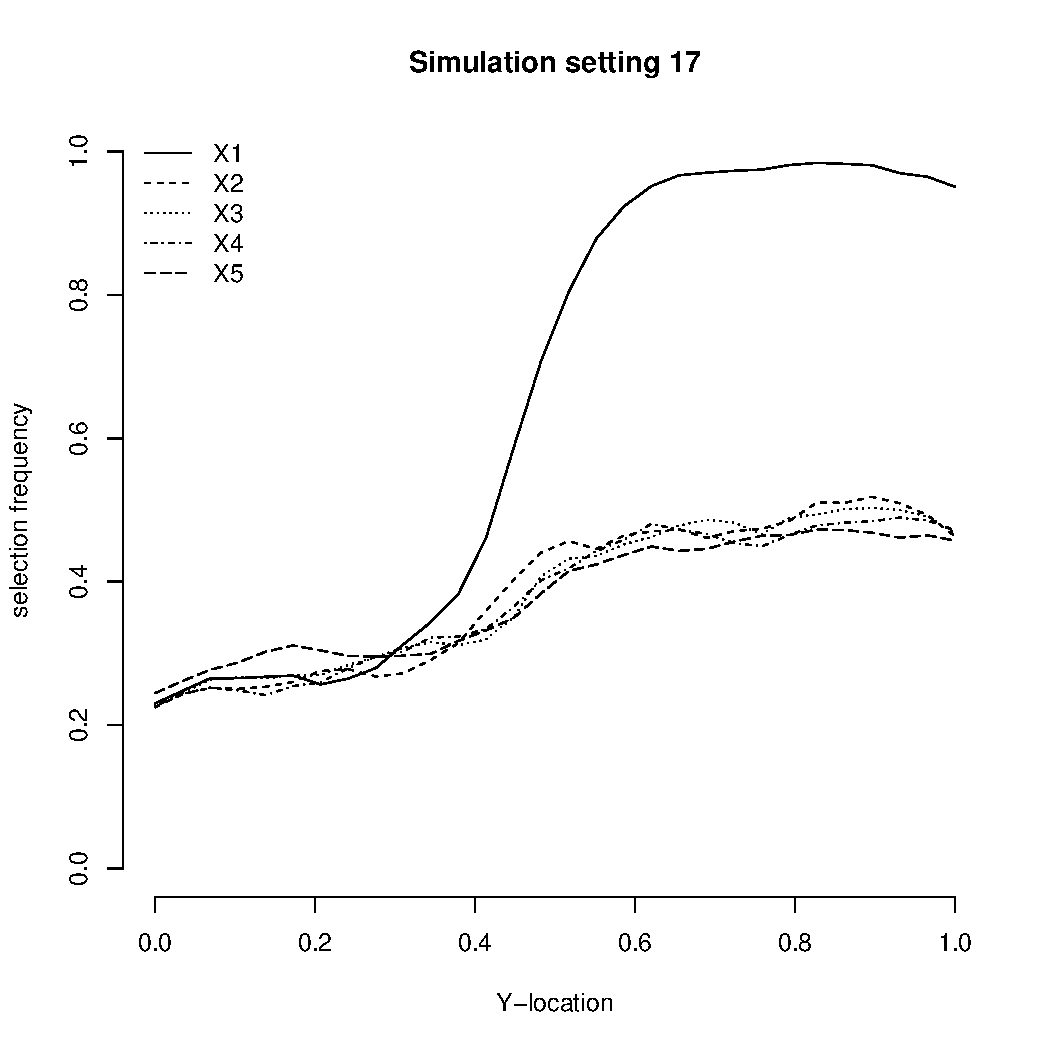
\includegraphics[width=\textwidth]{../../figures/simulation/28-17-profile-selection.pdf}
			%\caption{A tiger}
			\label{fig:tiger}
		\end{subfigure}
        ~ %add desired spacing between images, e. g. ~, \quad, \qquad etc.
          %(or a blank line to force the subfigure onto a new line)
		\begin{subfigure}[b]{0.3\textwidth}
			\centering
			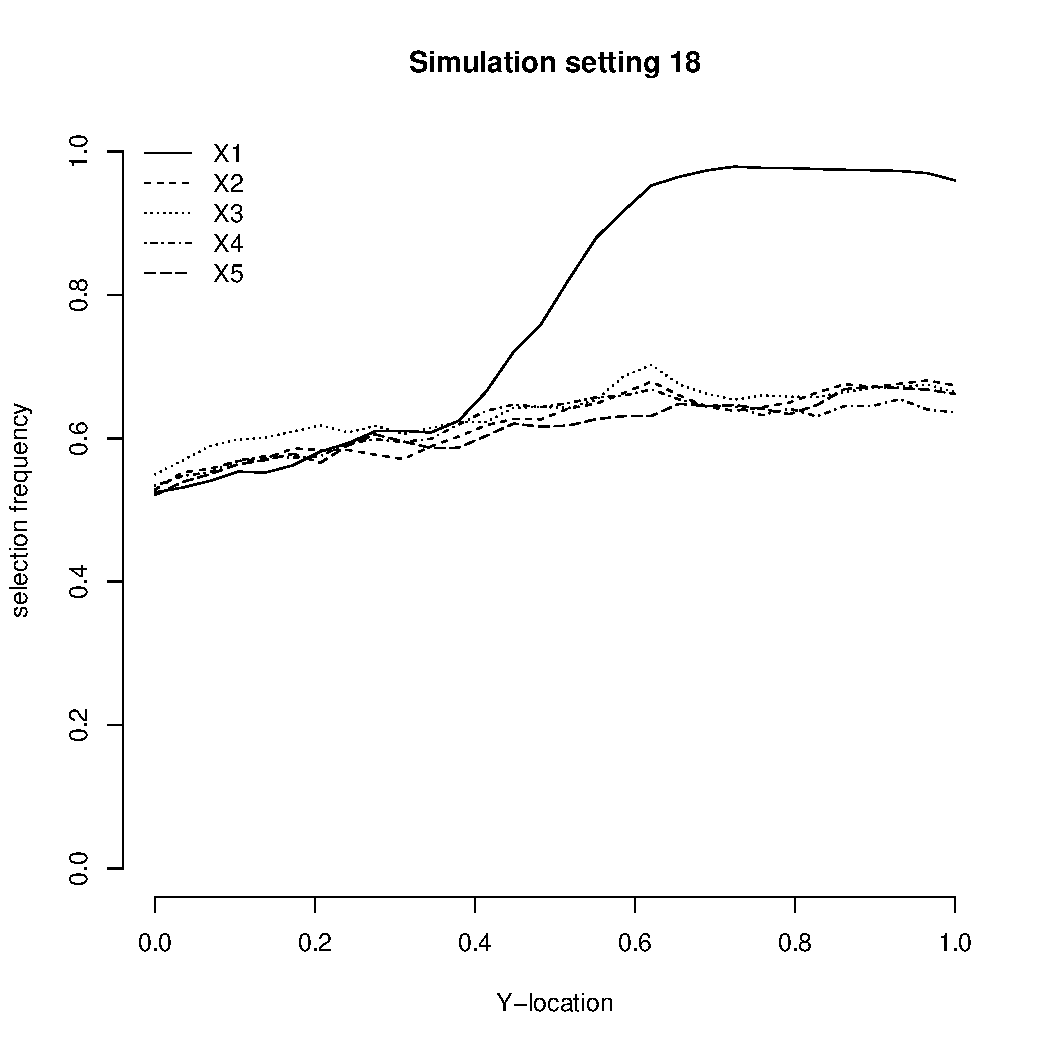
\includegraphics[width=\textwidth]{../../figures/simulation/28-18-profile-selection.pdf}
			%\caption{A mouse}
			\label{fig:mouse}
		\end{subfigure}
		%\caption{Pictures of animals}\label{fig:animals}
	\end{figure}	
		
\section{Data analysis}
	\subsection{Census poverty data}
	Data for this example comes from the U.S. Census Bureau's decennial census from 1960-2000, and from its American Community Survey in 2006. The variable being modeled is the logit of poverty rate by county in the states of Minnesota, Iowa, Wisconsin, Illinois, Indiana, and Michigan. A GWR model was fit to the data based on the predictors \verb!pag!, \verb!pex!, \verb!pman!, \verb!pserve!, \verb!pfire!, \verb!potprof!, \verb!pwh!, \verb!pblk!, \verb!phisp!, and \verb!metro!. One model was fit to the data from each census.
	
	\subsection{Figures}
	\begin{figure}
		\begin{center}
			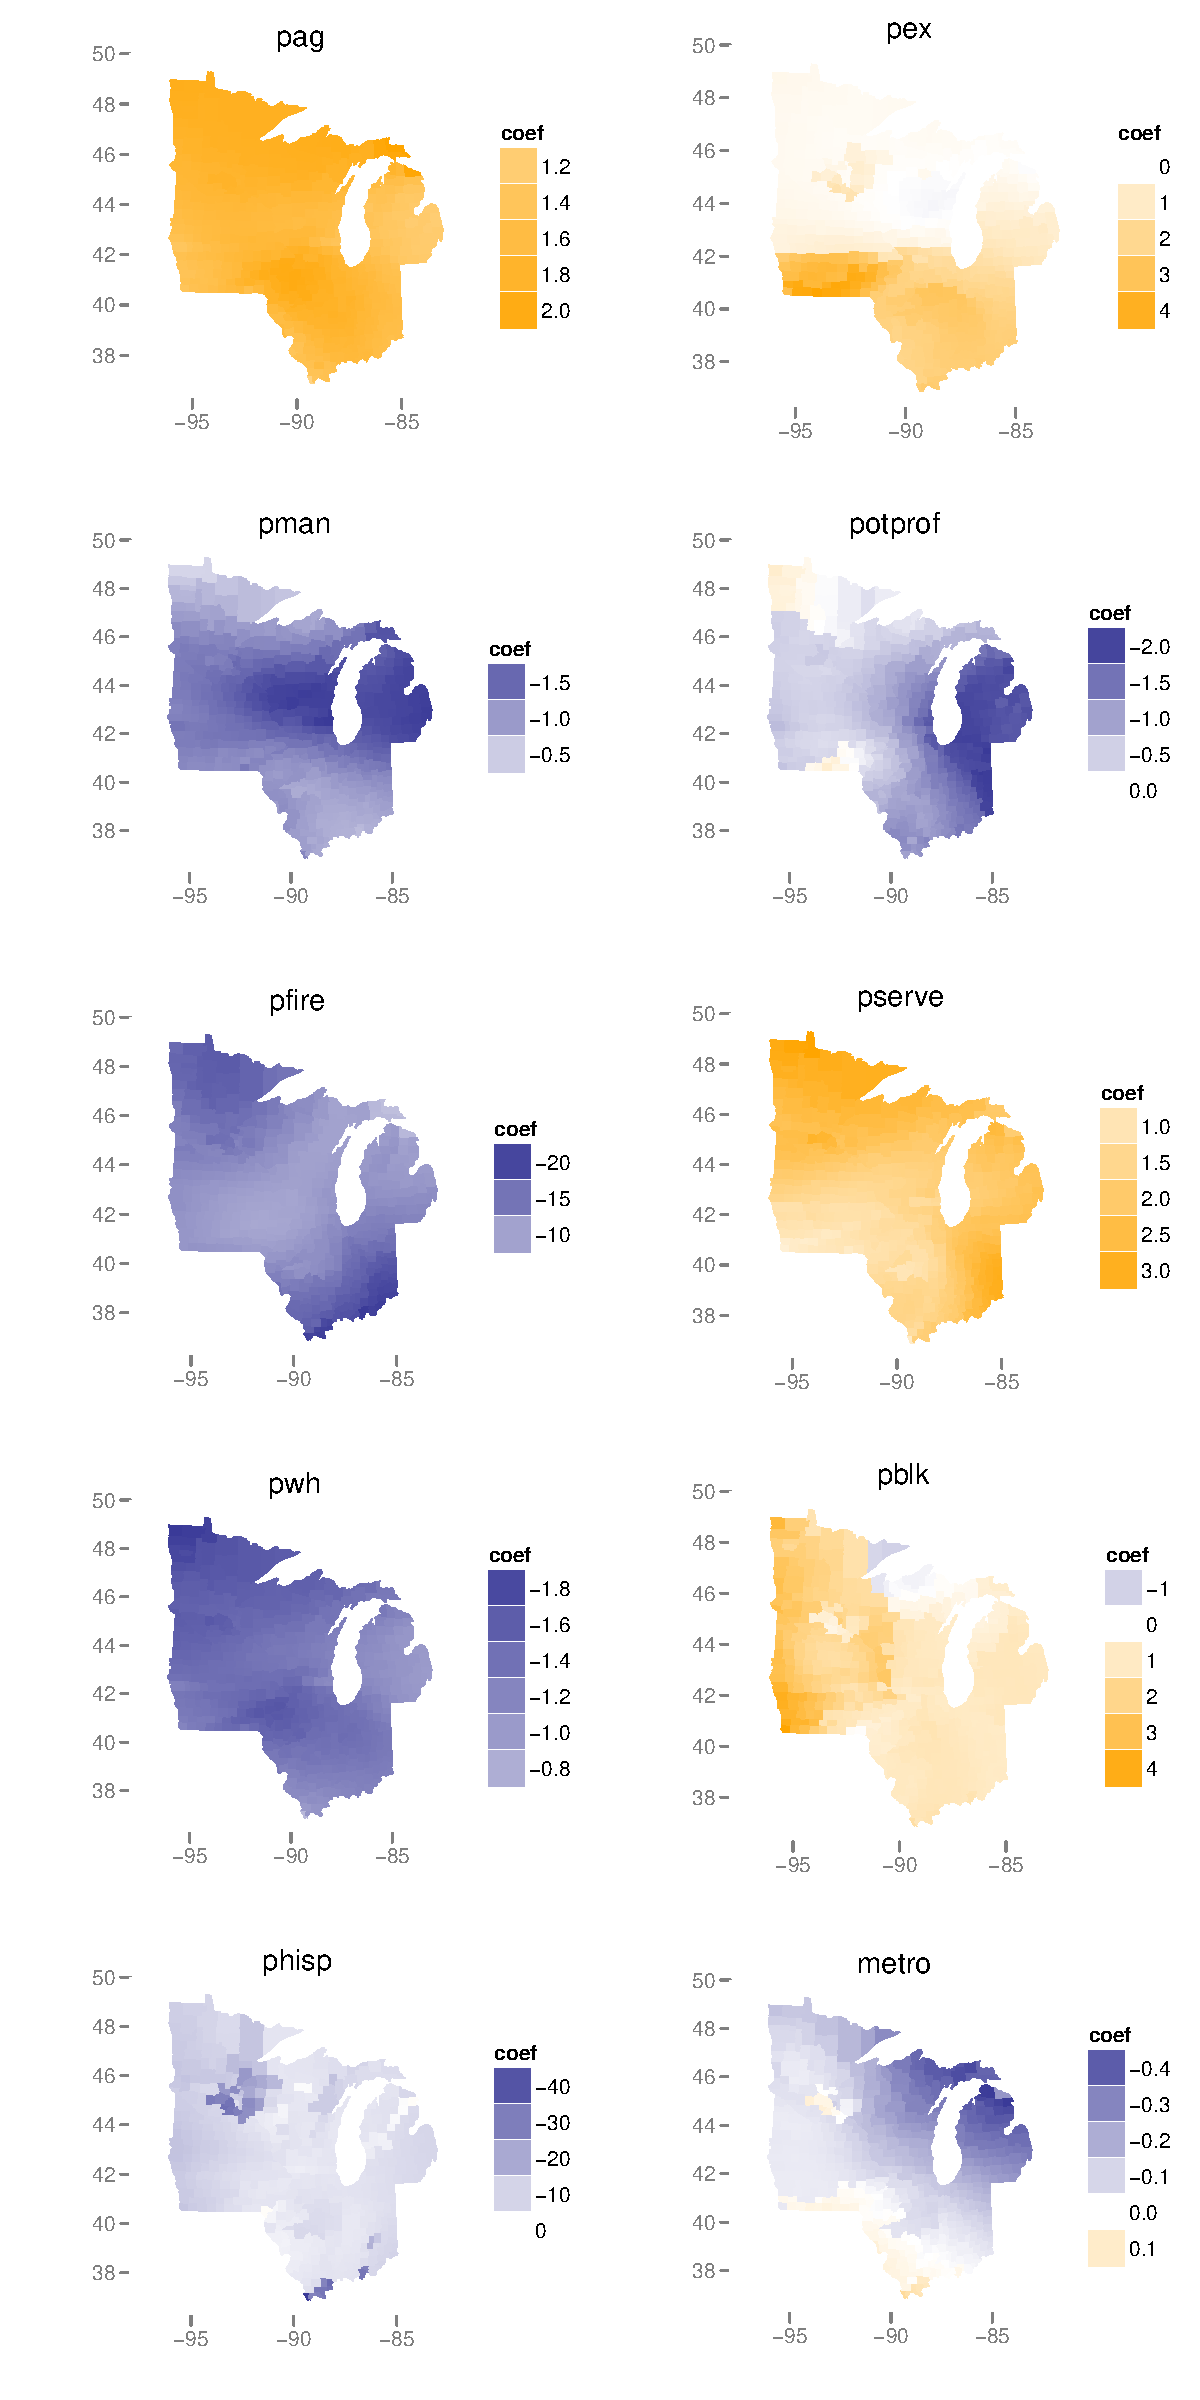
\includegraphics[height=8in]{../../figures/poverty/1960.linear.coefficients.pdf}
			\caption{Estimated coefficient surfaces for the 1960 census.\label{fig:1960}}
		\end{center}
	\end{figure}

	\begin{figure}
		\begin{center}
			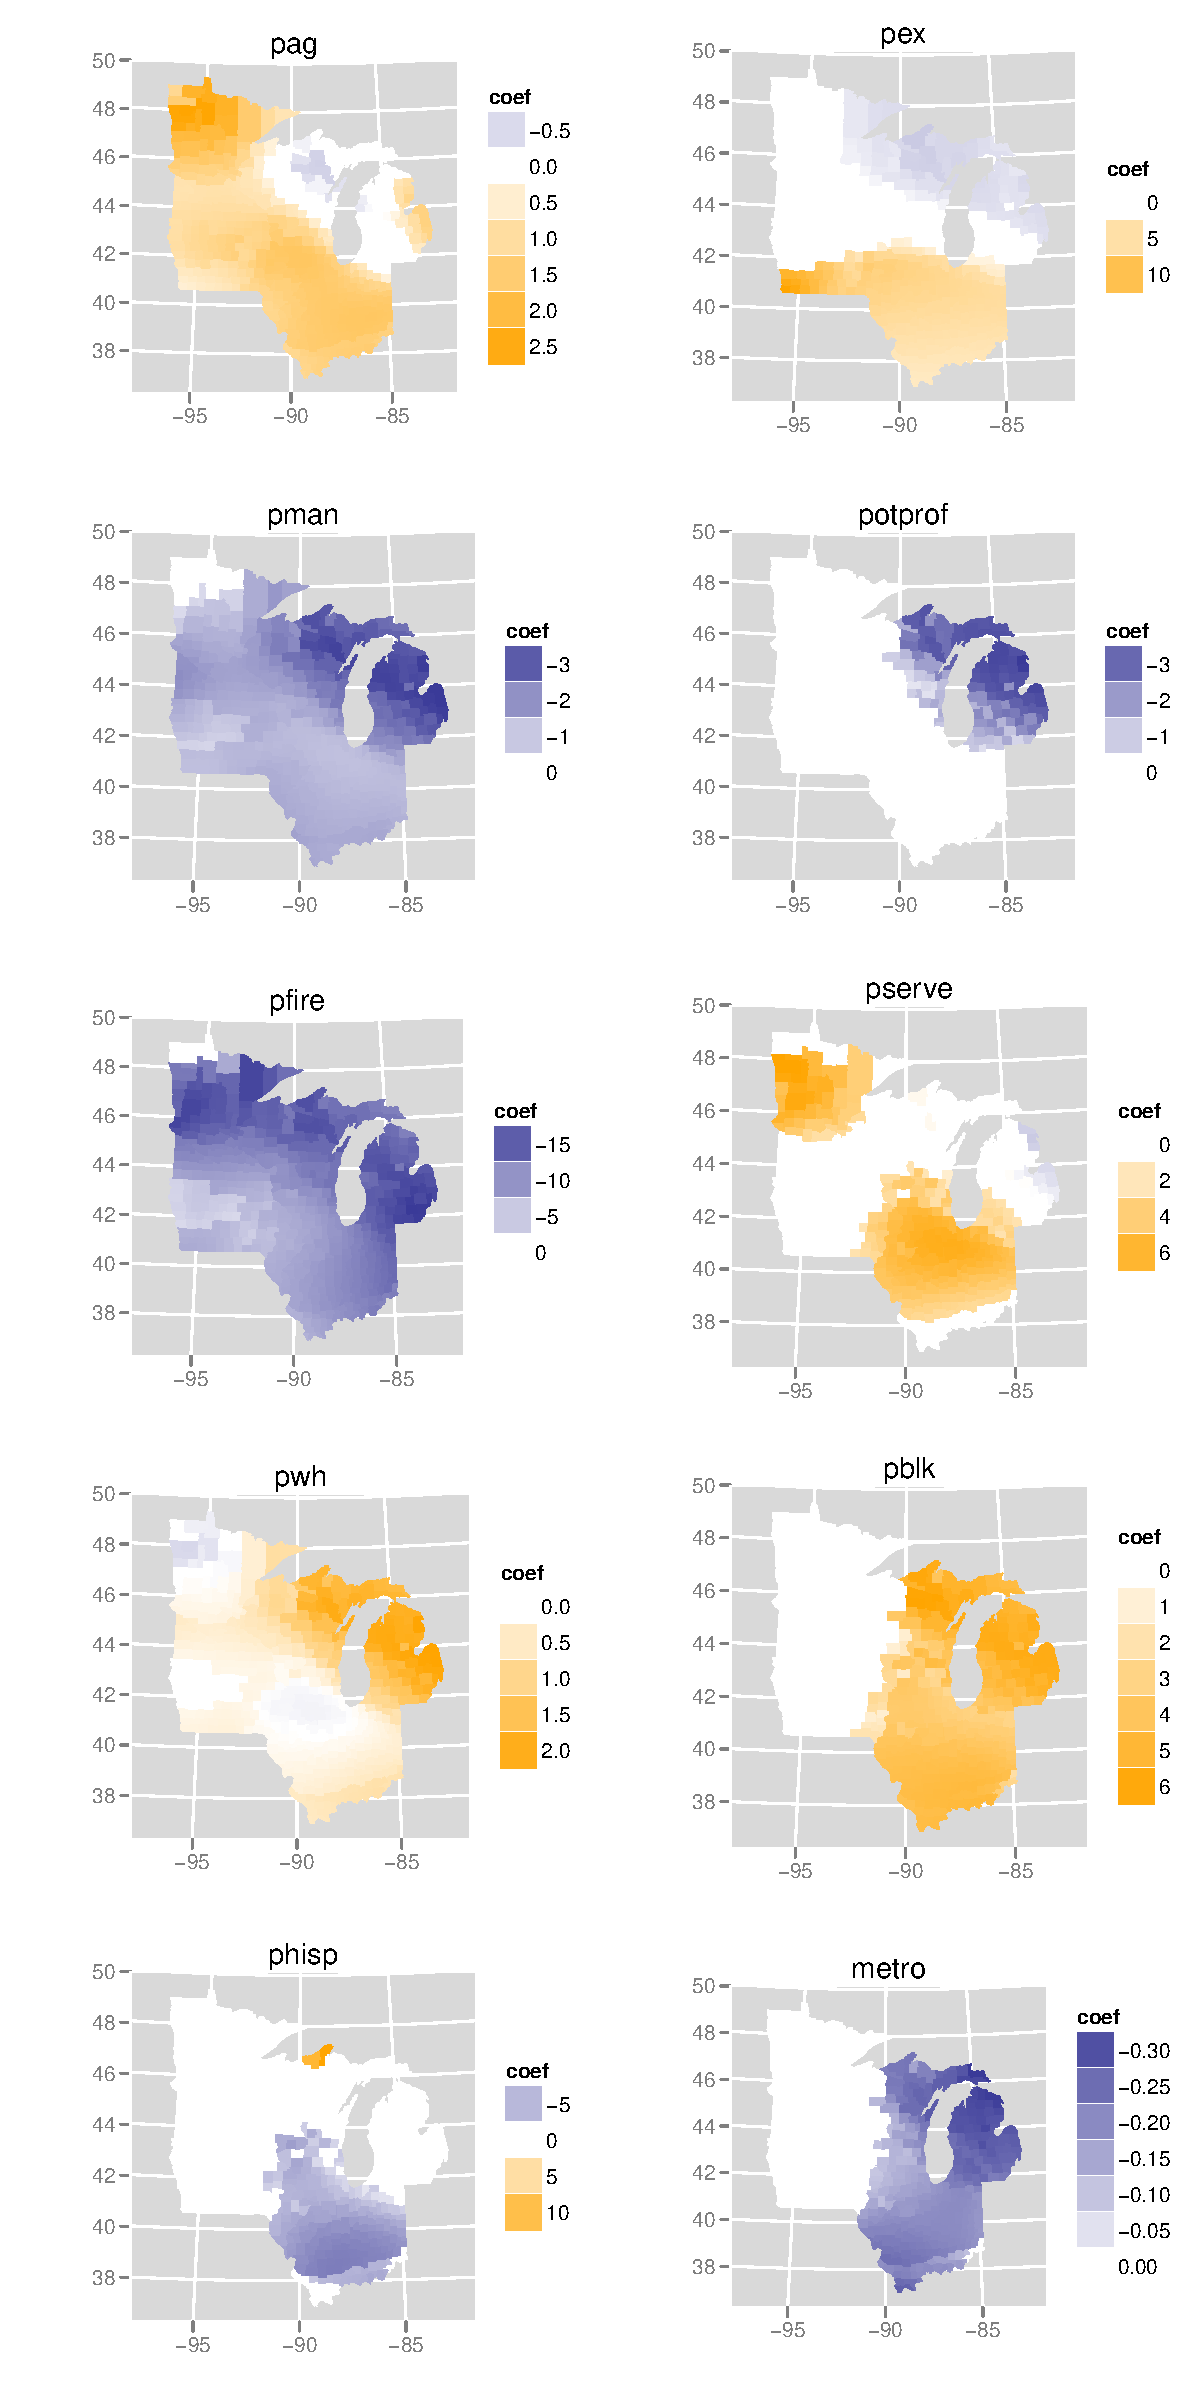
\includegraphics[height=8in]{../../figures/poverty/1970.linear.coefficients.pdf}
			\caption{Estimated coefficient surfaces for the 1970 census.\label{fig:1970}}
		\end{center}
	\end{figure}
	
	\begin{figure}
		\begin{center}
			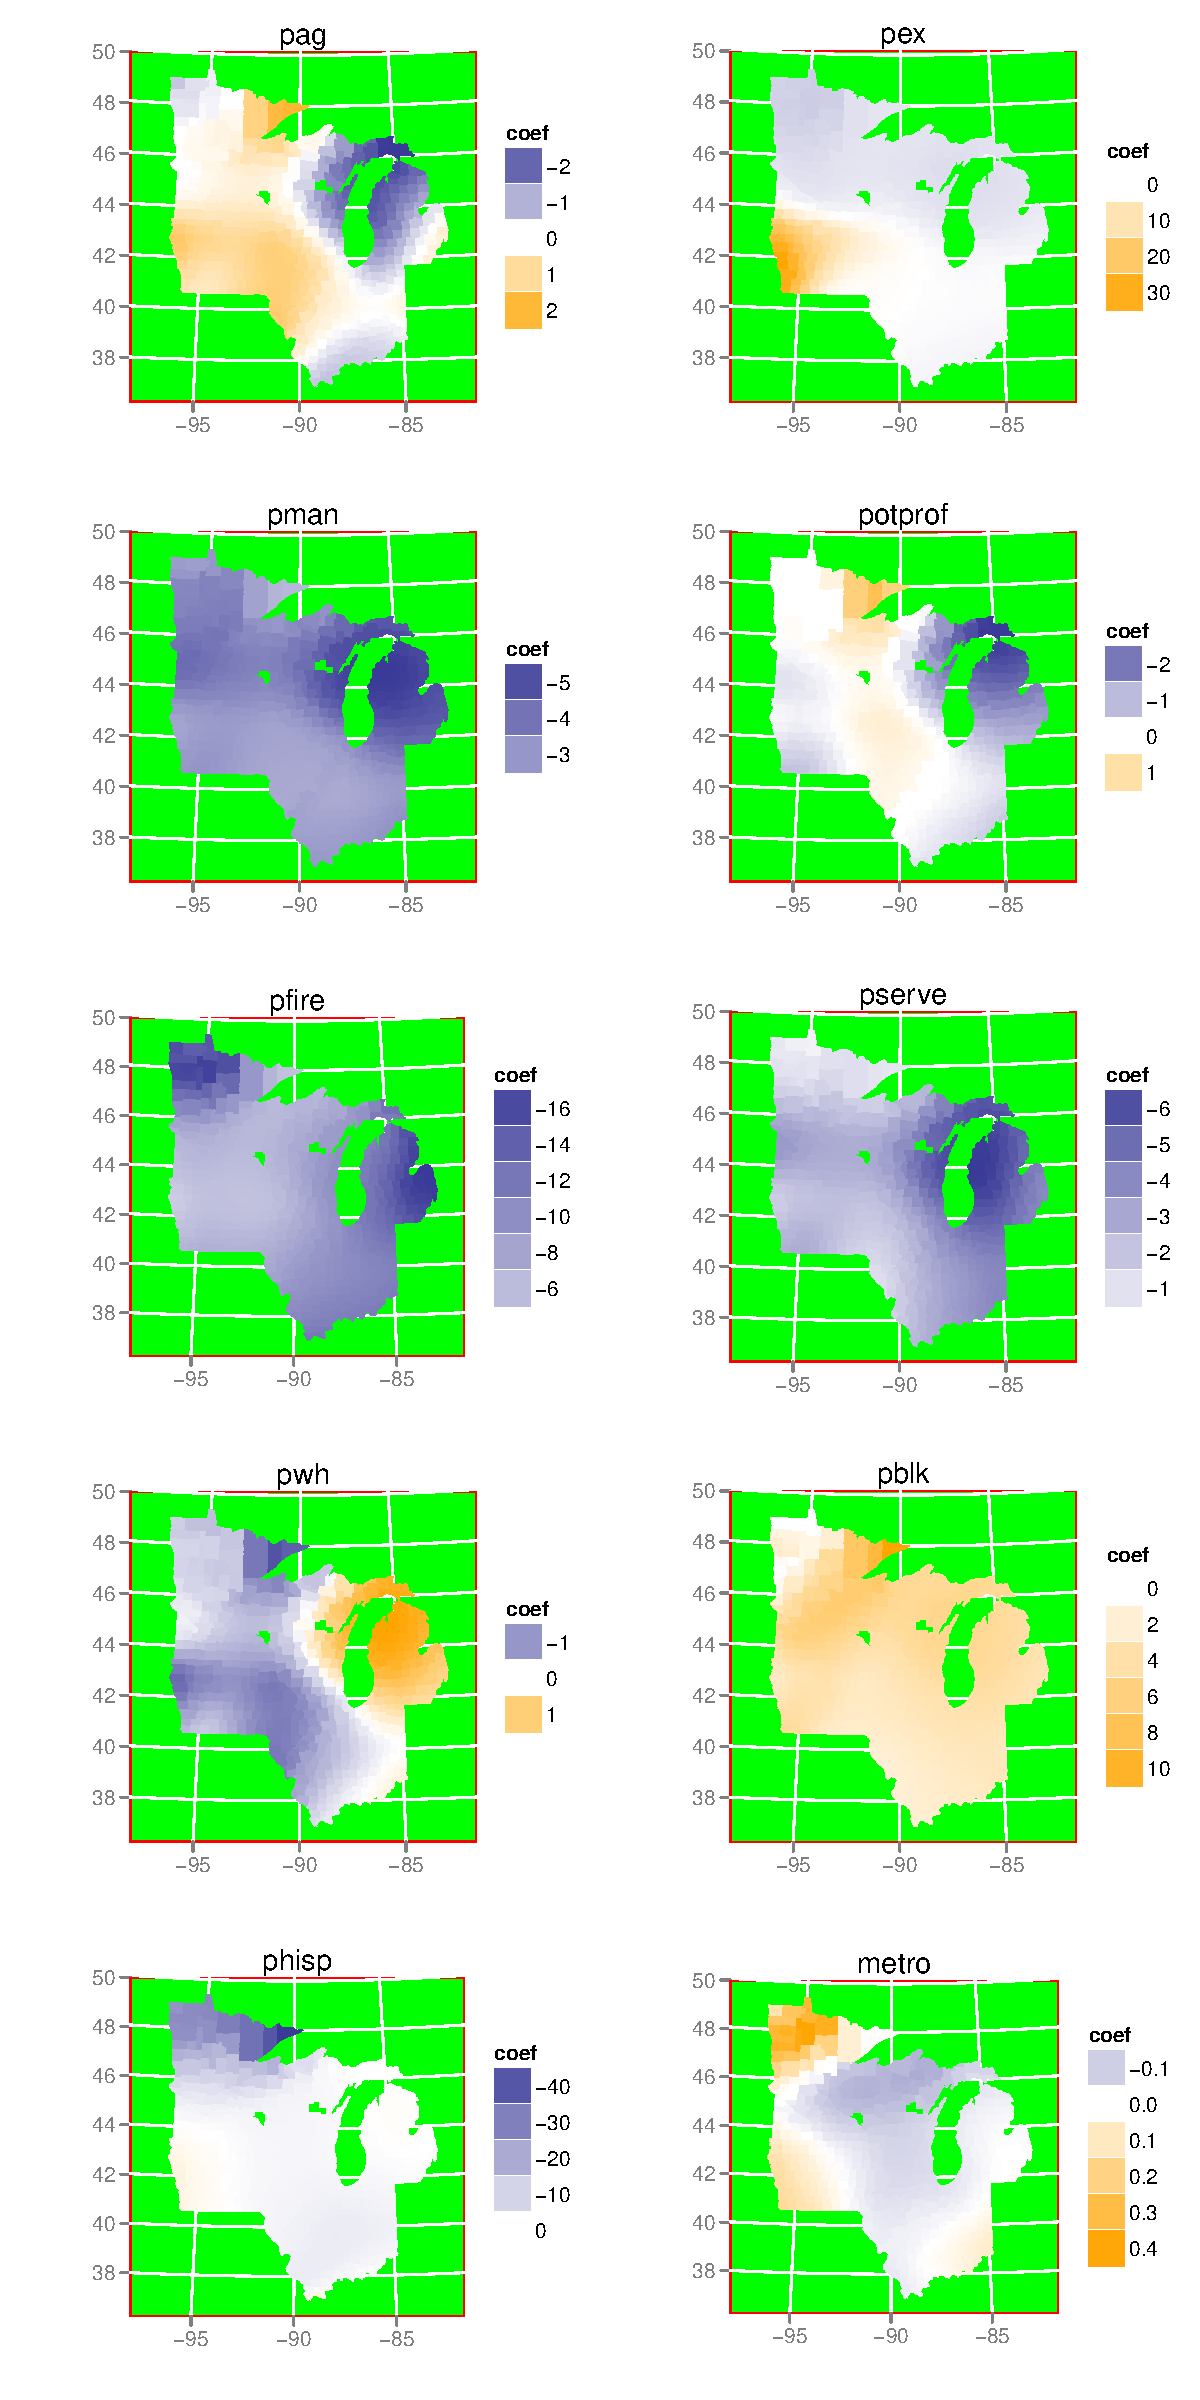
\includegraphics[height=8in]{../../figures/poverty/1980.linear.coefficients.pdf}
			\caption{Estimated coefficient surfaces for the 1980 census.\label{fig:1980}}
		\end{center}
	\end{figure}
	
	\begin{figure}
		\begin{center}
			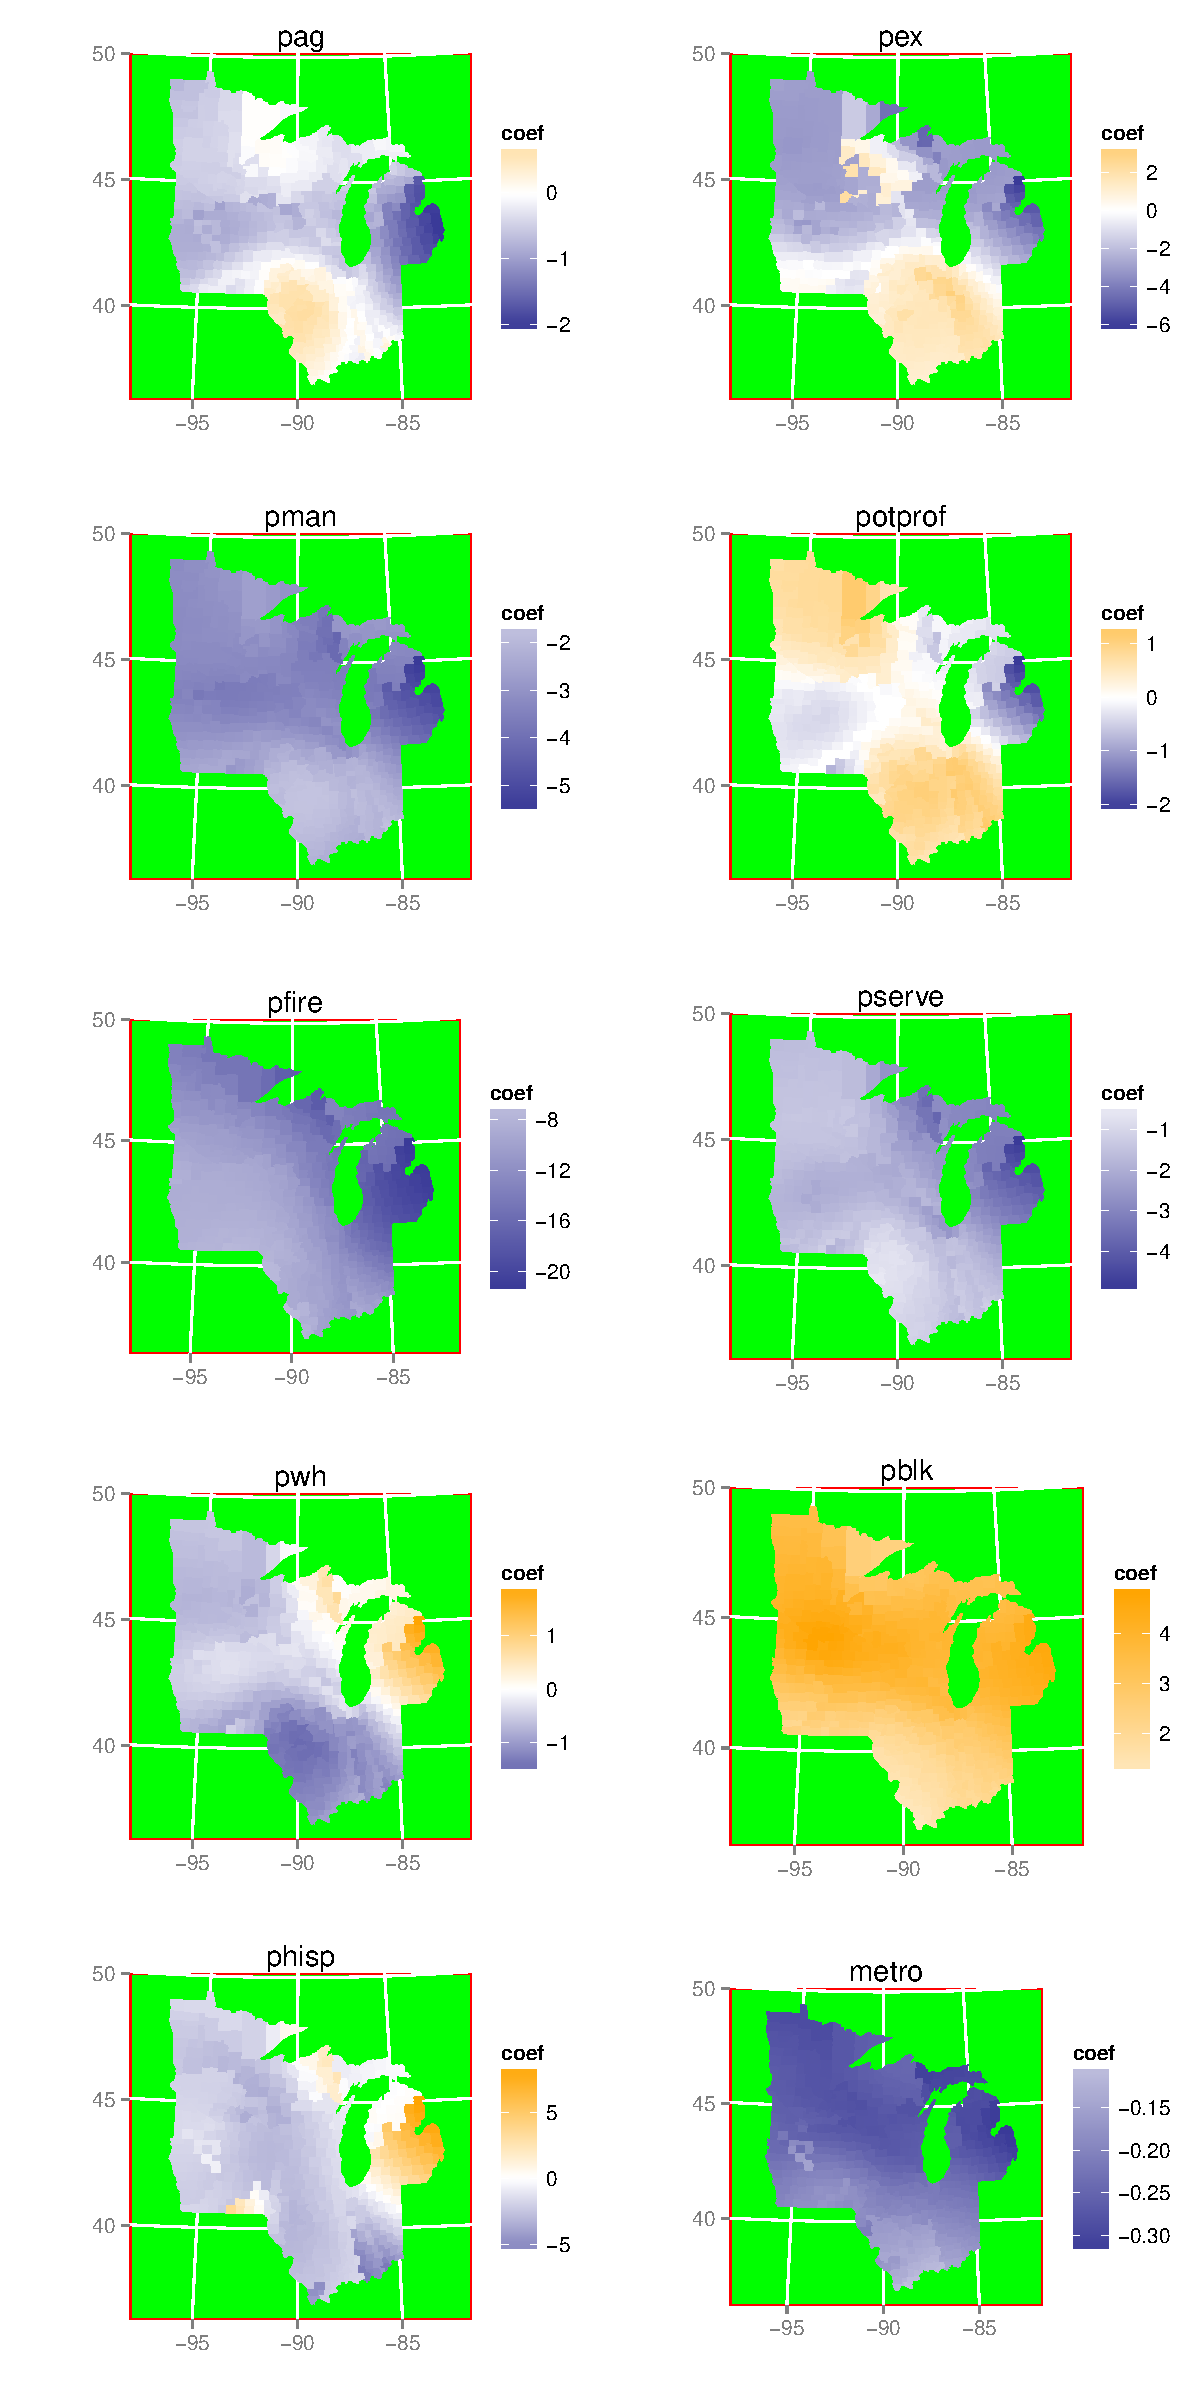
\includegraphics[height=8in]{../../figures/poverty/1990.linear.coefficients.pdf}
			\caption{Estimated coefficient surfaces for the 1990 census.\label{fig:1990}}
		\end{center}
	\end{figure}
	
	\begin{figure}
		\begin{center}
			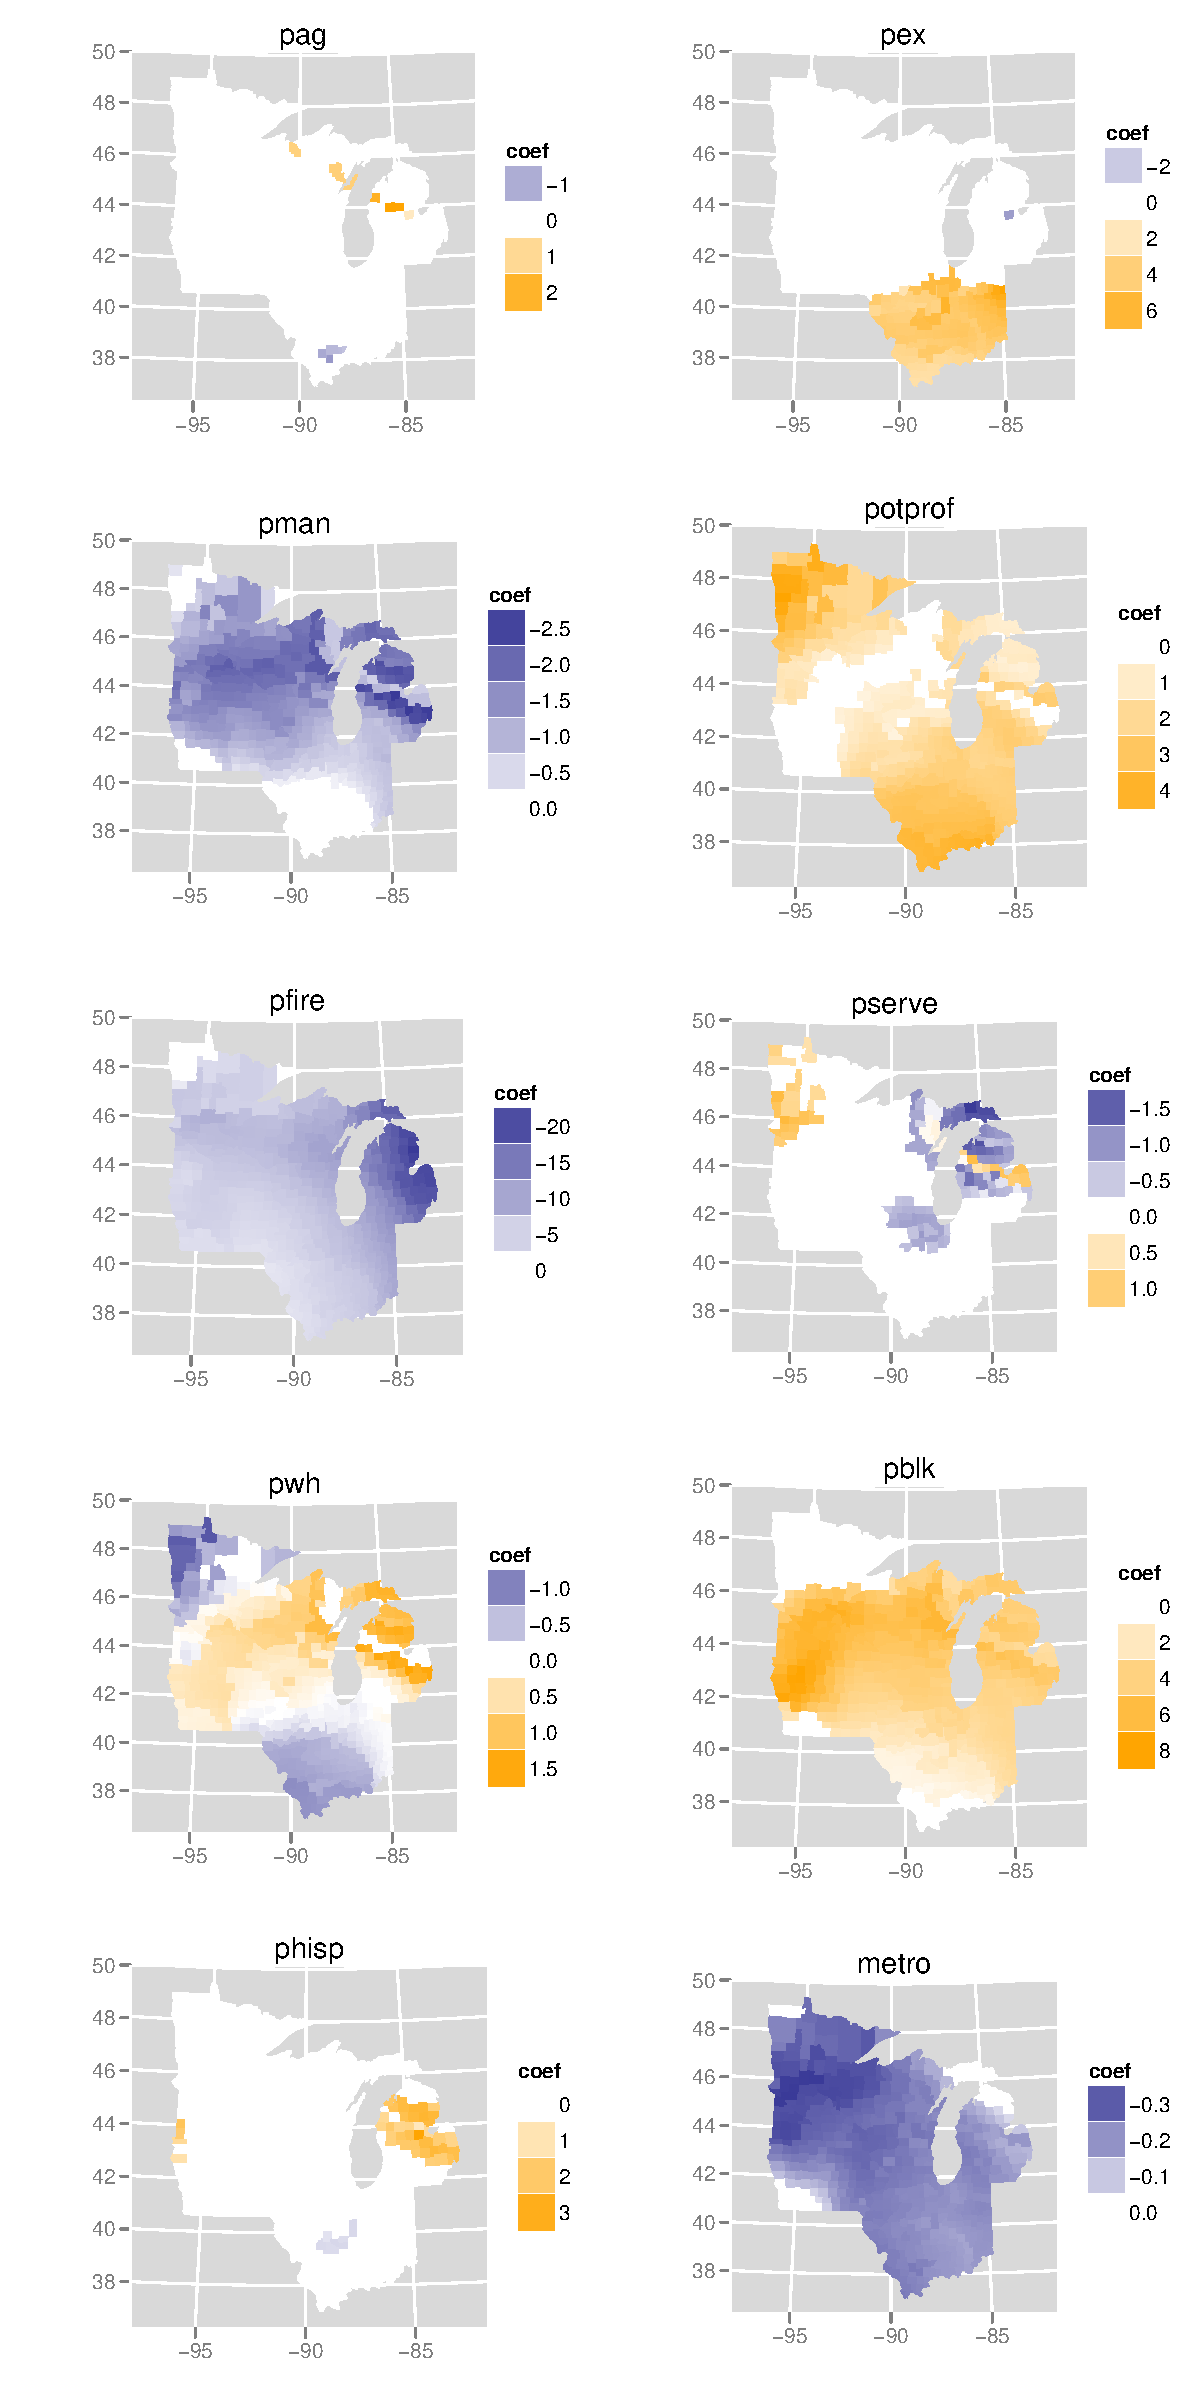
\includegraphics[height=8in]{../../figures/poverty/2000.linear.coefficients.pdf}
			\caption{Estimated coefficient surfaces for the 2000 census.\label{fig:2000}}
		\end{center}
	\end{figure}
	
	\begin{figure}
		\begin{center}
			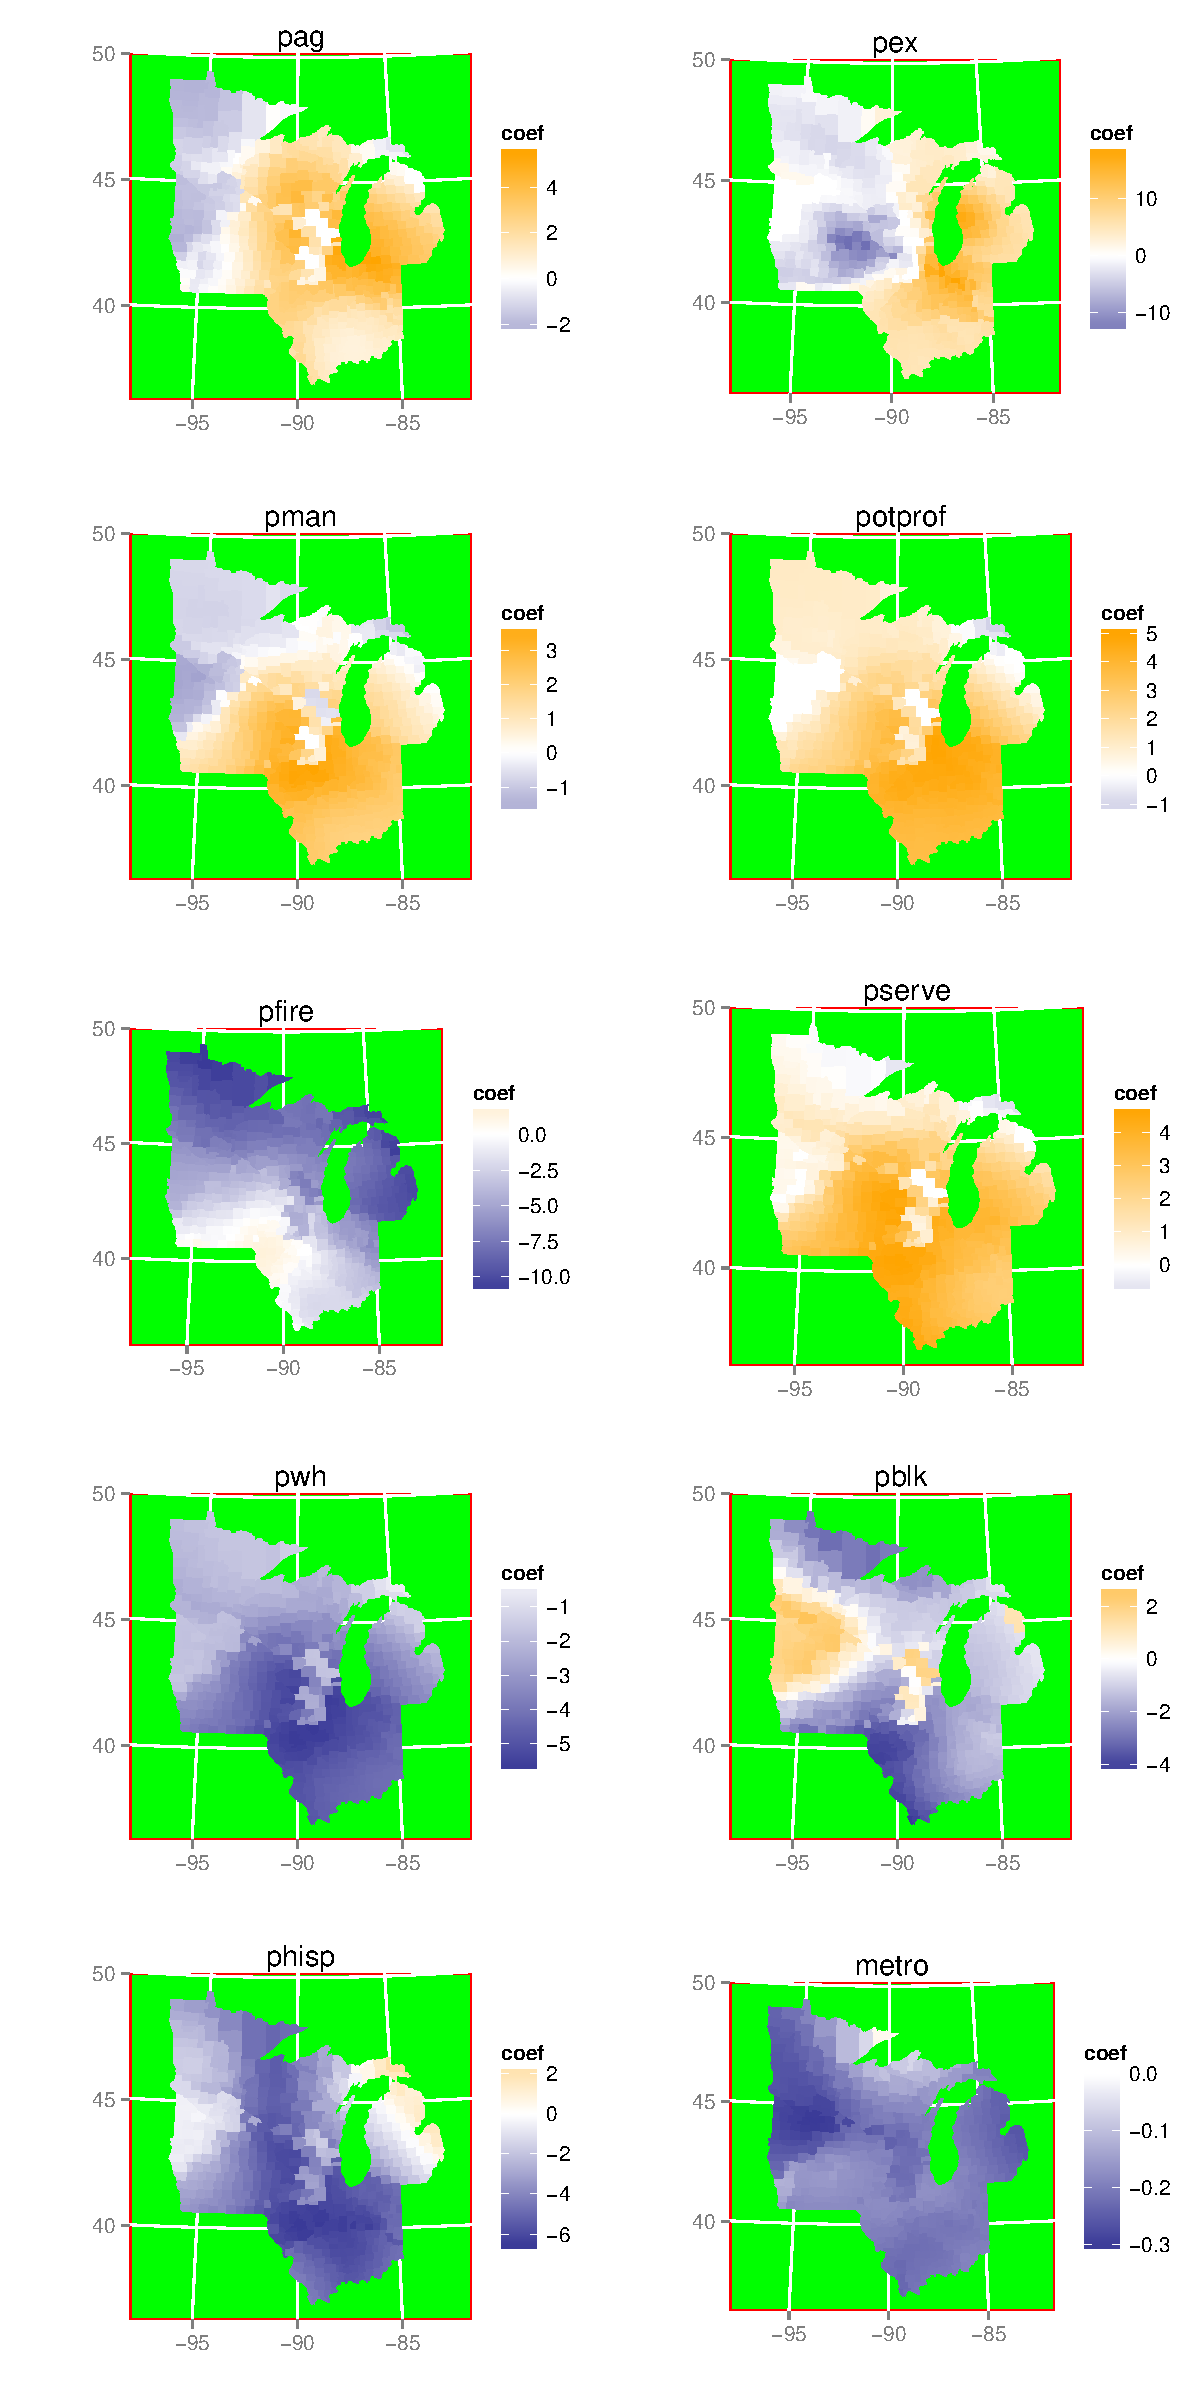
\includegraphics[height=8in]{../../figures/poverty/2006.linear.coefficients.pdf}
			\caption{Estimated coefficient surfaces for the 2006 census.\label{fig:2006}}
		\end{center}
	\end{figure}
			
\section{References}
\bibliographystyle{chicago}
\bibliography{../../references/gwr}

\end{document}  